\documentclass{rstb}

\usepackage[utf8]{inputenc}
\usepackage{amsmath}
%\usepackage{natbib}
%\usepackage[style=nature,citestyle=authoryear,natbib=true]{biblatex}

\usepackage{graphicx}
\usepackage{amsmath}
\usepackage{lineno}


\def\titlehead{Research}%%Please insert respective article type here
\Journal{Phil. Trans. R. Soc. B\ }
\begin{document}
\title{The Iron Law of Institutions: The co-evolution of institutions and hierarchy}
\author{Simon T.Powers$^{1}$, Cedric Perret$^{2}$ and Thomas E. Currie$^{2}$}
\address{$^{1}$Edinburgh Napier University, Edinburgh EH10 5DT\\ 
$^{2}$University of Exeter, Penryn TR10 9FE}
\subject{}
\corres{Simon T. Powers}
\begin{abstract}

Societies of all scales need to form institutional rules to regulate their social interactions. These specify, for example, what actions individuals should take in particular situations, and what sanctions will apply if individuals violate these rules. But forming these institutional rules involves playing a political game -- a process of negotiation and bartering between individuals that is costly and time consuming. Intuitively, this cost should be expected to increase as a group becomes larger, which could then select for a transition to hierarchy to keep the cost of playing the political game down as group size increases. However, previous work has lacked a mechanistic yet general model of political games that could formalise this argument and test the conditions under which it holds true. Here, we address this by formalising the political game using a standard consensus formation model. We show that the increasing cost of forming a consensus over institutional rules selects for a transition from egalitarian to hierarchical organisation over a wide range of conditions. Playing a political game to form institutional rules in this way captures and unites a previously disparate set of voluntary theories for hierarchy formation, and can explain why the increasing group size in the Neolithic would lead to strong hierarchy. 

% We show that this effect is controlled by the connectivity and the number of polities, and we find support for the idea that inequality tends to be lower in large open plains than in isolated valleys.

\end{abstract}
\keywords{Institutions, cooperation, hierarchy, punishment}

\rsbreak


\begin{linenumbers}
    

\section*{Introduction}
%Tom: Looking for some references and text on voluntary hierarchy theories, and how they amounts to forming rules
Societies of all scales, from hunter-gatherers to modern liberal democracies, are governed by institutional rules \cite{North:1990:a,Ostrom:1990:a} that help to promote cooperative behaviour and resolve social dilemmas \cite{Greif:2006:a,Singh:2017:a,Powers:2021:a}. For example, in the !Kung Bushmen, resource allocation is governed by a rule that says that the owner of the first arrow that penetrates the animal controls distribution after a cooperative hunt \cite{Testart:1987:a}, while in general hunter-gatherer societies have rules that regulate the conditions under which individuals should give food to others \cite{Kaplan:2009:a}. Likewise, agricultural societies have rules governing the usage and management of irrigation systems, specifying how much water an individual farmer may take and when, and how much they should contribute to maintaining the system \cite{Ostrom:1990:a,Guala:2012:a}. Moreover, in all scales of society these rules are enforced by graduated systems of monitoring and punishment \cite{Powers:2021:a}. These range from gossip and ridicule to hiding and ostracism in hunter-gatherers \cite{Boehm:1999:a}, through to third-party punishment by the state in liberal democracies.

Economics has long studied the effects that institutional rules have on incentivising cooperative social behaviour amongst self-interested agents (e.g. \cite{North:1990:a,Reiter:1996:a,Greif:2006:a}). Indeed, it is even  argued that the main determinant of whether a nation is poor or prosperous is the type of institutional rules governing the society, and whether these successfully incentivise cooperative division of labour and trade \cite{Acemoglu:2011:a}. A key research challenge, however, is understanding how institutional rules are formed and evolve. This is a key question for anthropology, archaeology, and evolutionary biology, which all seek to understand hows social behaviour, and hence institutional rules, change with the scale of a society. Yet despite the importance of this question, little work has been done in these disciplines in modelling and understanding the processes of institutional rule formation.

Some work has begun to address this by taking a game theoretic perspective to the evolution of institutional rules \cite{Powers:2013:a,Currie:2021:a,Gavrilets:2022:a}. This has drawn on work from economics that proposes a meta-model of institutional rule formation \cite{Hurwicz:1996:a,Reiter:1996:a}. This meta-model separates social interactions within a group into an economic game and a political game \cite{Powers:2016:a}. In the economic game, individuals have social interactions that directly affect their material payoff (calorie intake, size of shelter, etc.). Examples include choosing whether to join a cooperative hunting party, how much food to share with other group members, how much water to take from an irrigation system, and whether or not to pay taxes. This is the standard type of game studied in evolutionary anthropology, archaeology, and biology, and might be modelled as a public goods or prisoner's dilemma game, for example. However, in addition to this, group members also engage in a political game that sets the rules of this economic game. For example, how much water should each group member take from an irrigation system, how will this be monitored, and what will the sanctions be for taking more than the rules permit? The rules that result from the political game are known as the institutional rules, and determine the payoff matrix (or more formally, the game form, \cite{Hurwicz:1996:a}) of the economic game. Consequently, they determine the the extent to which self-interested individuals who are trying to maximise their material payoff will cooperate \cite{Greif:2006:a,Powers:2021:a}. An \emph{institution} is then defined as the set of possible rules that the individuals can choose between and implement, given the constraints that come from the laws of nature and the current state of their technology \cite{Hurwicz:1996:a}.

Political games essentially involve individuals bartering and negotiating over what the rules of their economic interactions should be \cite{Powers:2016:a}. This most obviously occurs in liberal democracies and states such as ancient Athens \cite{Ober:2008:a}, where formal assemblies debate over codified laws that govern economic interactions \cite{Reiter:1996:a}. But at the other end of the scale, hunter-gatherer societies spend a vast amount of time discussing the rules of their society and whether individuals are complying with them \cite{Boehm:1999:a}. The political game can therefore be more or less formal. Crucially, it may involve all or only a subset of group members. In egalitarian societies, most individuals might take part in negotiating over rules, while in hierarchical societies only the leader and their kin might take part. In either case, we would expect individuals to try and influence the political game to produce rules that will benefit themselves. In other words, individuals will have a strategy in the political game, i.e. a preference for the rules that they would like to see be implemented. Note that we do not need to assume that individuals are fully rational and completely aware of the consequences of their decisions to be able to play a political game in this way. Trial-and-error, or cultural evolution through payoff-biased social learning \cite{Boyd:1985:a}, will over time lead individuals to adopt strategies in the political game that produce rules which increase their material payoff in the economic game. 

However, previous work has largely ignored the cost to individuals of playing the political game. Playing a political game -- bartering and negotiating over rules -- clearly carries an opportunity cost for the individuals involved. Simply put, time spent negotiating and trying to convince others is time that could otherwise be spent on productive economic activities such as hunting, fishing or farming (i.e. playing the economic game for material payoff). Moreover, in an egalitarian group we would expect this cost of playing the political game to increase as the size of the group increases, because more individuals would need to come to a consensus over what the rules should be. This is an instance of the general phenomenon known as scalar stress \cite{Johnson:1982:a} -- as group size increases, coordination problems such as deciding on institutional rules become more difficult to solve. In political science, the ``Iron Law of Oligarchy'' suggests that as groups become larger, they inevitably end up switching from egalitarian to hierarchical organisation to overcome these problems and be able to make and enforce decisions efficiently \cite{Michels:1911:a}. The anthropological and archaeological evidence for the evolution of human societies also shows this pattern. As societies increased in size following the origin of agriculture and the Neolithic Demographic Transition \cite{Bocquet-Appel:2011:a}, they switched from egalitarian to hierarchical organisation \cite{Boehm:1999:a,Price:1995:a,Price:2010:a}. And even in modern liberal democracies, only a small subset of individuals -- the elected representatives -- spend their time negotiating over institutional rules.

In this paper, we examine the hypothesis that as group size increased during the Neolithic, the process of playing the political game to negotiate institutional rules became more and more costly for egalitarian groups. This could then select for a transition to hierarchical organisation to allow groups to continue to grow in size while reducing the cost of rule formation. If correct, this hypothesis would provide a general explanation for why groups switch to hierarchy as their size increases, since practically every group needs to form rules to regulate their social interactions \cite{North:1990:a,Fukuyama:2011:a}, and the number of such rules increases with the size of the group (e.g. the small-scale Kapauku Papuan society has around 120 rules regulating areas from property rights through to punishment for murder, whereas 40,000 new laws took effect in the United States in 2014 alone \cite{Singh:2017:a}). In particular, most cases of `functional' or `integrative' theories for the evolution of hierarchy \cite{Calvert:1992:a,vanVugt:2006:a,King:2009:a,Hooper:2010:a,Sterelny:2013:a} are actually examples of playing a political game to form rules (e.g. deciding rules over construction of irrigation systems \cite{Wittfogel:1957:a,Nichols:1993:a,Spencer:1993:a,Carballo:2014:a}, harvesting of marine resources \cite{Arnold:1995:a,Friesen:1999:a,Alvard:2002:a}, or defensive warfare \cite{Boone:1992:a,Roscoe:2013:a}). 

To be able to address this, we need a model of the political game that is general enough to capture many cases of rule formation, while being mechanistic enough to demonstrate how the cost of rule formation increases with group size. In previous work, political games have generally been modelled very abstractly in a way that does not allow the relationship between their cost and group size to be analysed. Some models have only considered institutional rules as group-level traits that change by unspecified (effectively random) processes within groups followed by group competition \cite{Turchin:2013:a,Richerson:2016:a}. Other models have captured the political game within a group as simply taking the mean preference of the group members \cite{Powers:2013:a,Powers:2017:a}, or taking a majority vote \cite{Currie:2021:a}. None of these are detailed enough to show how the cost of rule formation scales with group size. 

Here, we overcome this limitation by using a standard consensus formation model \cite{Gavrilets:2016:a,Perret:2022:a} to capture the political game. In a consensus formation model, individuals start with an initial opinion, and then modify this based on interactions with other individuals until a consensus is reached where the variance of their opinions is less than some threshold. How much individuals sway the consensus towards their own opinion depends on their influence relative to the influence of other individuals -- the consensus is closer to the opinion of individuals with higher influence. In an egalitarian group, each individual would have roughly the same influence, while in a hierarchical group leaders would have a higher influence than followers. Crucially, the time it takes to reach consensus depends on the distribution of influence -- if all individuals have similar influence, i.e. the group is egalitarian, then it will take longer to reach consensus than if a few individuals have much higher influence, i.e. the group is hierarchical \cite{Gavrilets:2016:a,Perret:2020:a}. Moreover, previous work has shown that consensus time increases with group size, and at a faster rate in egalitarian compared to hierarchical groups \cite{Perret:2020:a}.

By considering the influence of an individual as an evolvable trait, and considering the time to reach consensus as an opportunity cost of playing the political game that is subtracted from individual fitness, we can demonstrate conditions under which evolution will lead to egalitarian or hierarchical organisation in response to the demands of rule formation. To do this, we build on an existing model of the co-evolution of institutions, demography and cooperation during the Neolithic \cite{Powers:2013:a}. This demonstrated conditions under which institutional rules for punishment co-evolved with group size to support the transition from small-scale to large-scale cooperative groups. However, it considered a fixed cost of playing the political game, which was an exogeneous parameter. Here, we replace that abstract model of the political game with a consensus formation model, and also allow individuals to evolve their influence. This allows us to demonstrate that as a group grows in size from the benefits of cooperation (e.g. constructing an irrigation system), the increasing costs of institutional rule formation select for individuals to evolve hierarchy under a wide range of conditions. This matches the archaeological and anthropological evidence of societal evolution from the Neolithic, and provides formal support for the ``Iron Law of Oligarchy''.

\section*{Model description}
Our model builds upon the model of the co-evolution of institutions, demography and large-scale cooperation presented in \cite{Powers:2013:a}. In that model, individuals live on a number $N_\mathrm{p}$, of resource patches connected by migration, and can be either social or asocial. Social individuals agree to form an institution on their patch, and then play a public goods game regulated by the institutional rules. Asocial individuals, on the other hand, do not take part in institution formation or the public goods game. The inclusion of asocial individuals allows the model to demonstrate the origin of an institution, by showing conditions under which self-interested individuals would choose to form an institution. The institutional rules, $p_j$, specify how much of the public good generated by social individuals on their patch $j$ is invested into monitoring and punishment of defectors -- individuals who do not cooperate in the public goods game. The remaining share of their public good, $1-p_j$, is then invested into producing technology that increases the carrying capacity of all social individuals on the patch, e.g. an irrigation system. In \cite{Powers:2013:a}, the institutional rules $p_j$ were formed by taking the mean preference of all social individuals on the patch, and all social individuals payed a fixed opportunity cost $I$ for doing this compared to asocials. This represented the political game. 

The results were that if patches started off at a small size (around 20 individuals) then social individuals could invade a population of asocials, and evolved to create institutional rules that selected for high levels of cooperation. Specficially, individuals evolved their own preferences for the rules to invest most of their public good into technology that raised their carrying capacity, while investing just enough (around 15 to 20 percent) into monitoring and punishment to prevent defection in the public goods game from being individually advantageous. This occured because individuals in patches with these kinds of rules had more offspring compared to both asocials, and compared to individuals on patches with other institutional rules that invested either so much into monitoring and punishment that they lost the benefits of producing technology, or so little that social defectors outcompeted cooperators. Groups with these optimal instituitional rules then grew in size (up to hundreds of individuals) due to technology increasing their carrying capacity, capturing the demographic transition from small to large groups that occurred during the Noeolithic.

We now go on to provide a complete specification of the model, focusing on how we reimplement the political game with a consensus formation model, and on how we now allow individuals to evolve their influence, and hence the level of hierarchy on their patch.

%, alongside whether they are asocial, a social cooperator, or a social defector, and their preference for the institutional rules.

\subsection*{Lifecycle and population structure}

The lifecycle and population structure follows that in \cite{Powers:2013:a}. The population is subdivided into a finite number, $N_\mathrm{p}$, of resource patches, that are connected by migration following Wright's finite island model of dispersal \cite{Wright:1931:a}. The lifecycle of individuals consists of discrete and non-overlapping generations, as follows. (1) Local interactions occur on each patch, with social individuals forming institutional rules and playing a public goods game in which they can either cooperate or defect. (2) Each individual $i$ on patch $j$ has a Poisson distributed number of offspring that survive to adulthood, with the mean of the distribution being determined by the local social interactions and resource abundance (defined explicitly below). (3) Adults of the previous generation perish. (4) Each individual of the descendant generation either remains on its local patch (with probability $1-m$) or disperses to a randomly chosen patch (excluding the natal one). 

\subsection*{Evolving traits}

Individuals carry three cultural traits that are transmitted vertically from parent to offspring. This kind of transmission of cultural traits such as preferences and values from parents to offspring is common in both hunter-gatherer groups \cite{Hewlett:2011:a} and modern societies \cite{Cavalli-Sforza:1981:a}. The first trait, $\tau_{ij}$, is discrete and determines the social type of the individual. That is, whether the individual is \emph{asocial}, $\tau_{ij}=\mathrm{a}$ (does not take part in institution formation, receive no public good, and are not sanctioned), a social \emph{cooperator}, $\tau_{ij}=\mathrm{c}$ (takes part in institution formation and cooperates in the public goods game), or a social \emph{defector}, $\tau_{ij}=\mathrm{d}$ (takes part in institution formation but defects in the public goods game by not contributing). Mutation occurs on this trait with probability $\mu_\mathrm{\tau}$ by switching to one of the other two values chosen at random.

The second trait, $p_{ij}$, determines the intrinsic preference that the individual has for the institutional rules, specifically, the proportion of the public good on its patch that it thinks should be used to pay for the monitoring and punishment of defectors, as opposed to invested in technology. This trait is continuous in the range $[0,1]$. 

In this paper we add a third trait, $\alpha_{ij}$, which determines the influence of the individual in the consensus formation process (political game). This is also continuous in the range $[0,1]$. A larger value of $\alpha_{ij}$ means that the individual is more stubborn and persuasive when discussing with other individuals about what the institutional rules should be \cite{Gavrilets:2016:a,Perret:2020:a,Perret:2022:a}. For both $p_{ij}$ and $\alpha_{ij}$, mutation changes the trait value according to a truncated normally distributed random variable (with variance $\sigma$), centered around the current trait value. Mutation occurs on these traits with probabilities $\mu_\mathrm{p}$ and $\mu_\mathrm{\alpha}$, respectively. We assume a higher mutation rate for $p_{ij}$ than for the other traits. Asocials carry the $p_{ij}$ and  $\alpha_{ij}$ traits, but do not express them. 

\subsection*{Individual fitness}
Following \cite{Powers:2013:a}, the expected number $w_{\tau j}(t_\mathrm{g})$ of offspring that survive to adulthood (fitness) produced by an individual of type $\tau \in\{\mathrm{a},\mathrm{c},\mathrm{d}\}$ (asocial, cooperator, and defector, respectively) in patch $j$ at time $t_\mathrm{g}$ (where the subscript $g$ denotes generational time) is assumed to follow a discrete time Beverton-Holt model (e.g. \cite{Chow:2012:a}) with two niches, social and asocial. The degree of competition between these niches is set by two parameters, $\eta_{\mathrm{as}}$ and $\eta_{\mathrm{sa}}$, which give the per capita effect of socials on asocials' fitness, and asocials on socials' fitness, respectively. According to these assumptions, we write the fitnesses of the three types on patch $j$ at time $t_\mathrm{g}$ as
\begin{linenomath}
\begin{align}
\label{eqnwl}
w_{\mathrm{a}j}(t_\mathrm{g}) &= \frac{r_{\mathrm{a}}}{1 + n_{\mathrm{a}j}(t_\mathrm{g})/K_\mathrm{a}+\eta_{\mathrm{as}}\left[n_{\mathrm{c}j}(t_\mathrm{g})+n_{\mathrm{d}j}(t_\mathrm{g})\right]}  \nonumber\\
w_{\mathrm{c}j}(t_\mathrm{g}) &= \frac{r_{\mathrm{c}}}{1 + \left[n_{\mathrm{c}j}(t_\mathrm{g})+n_{\mathrm{d}j}(t_\mathrm{g}) \right]/K_{\mathrm{s}j}(t_\mathrm{g}) +\eta_{\mathrm{sa}}n_{\mathrm{a}j}(t_\mathrm{g})}\nonumber\\
w_{\mathrm{d}j}(t_\mathrm{g}) &= \frac{r_{\mathrm{d}j}(t_\mathrm{g})}{1 + \left[n_{\mathrm{c}j}(t_\mathrm{g})+n_{\mathrm{d}j}(t_\mathrm{g})\right]/K_{\mathrm{s}j}(t_\mathrm{g}) +\eta_{\mathrm{sa}}n_{\mathrm{a}j}(t_\mathrm{g})}, 
\end{align}
\end{linenomath}
where $n_{\tau j}(t_\mathrm{g})$ is the number of individuals of type $\tau$ on patch $j$ at time $t_\mathrm{g}$. The numerator in each expression can be thought of as the maximal growth rate of an individual of the corresponding type, while the denominator as the intensity of density-dependent competition faced by that individual. This Beverton-Holt fitness model is demographically explicit, and so allows us to capture the feedback between group size and cooperation, institutional rules and hierarchy. 

We now detail the parameters in the above fitness functions.

\subsection*{The economic game: Cooperation and institutionally-arranged punishment}
First, $r_{\mathrm{a}}$  ($\geq 0$) is the maximal growth rate of an asocial type. The maximal growth rate of a cooperator is assumed to be given by
\begin{linenomath}
\begin{align}
r_{\mathrm{c}}&=r_{\mathrm{a}} -\iota_j(t_\mathrm{g}) -C \label{eqnrc},
\end{align}
\end{linenomath}
where $\iota_j(t_\mathrm{g})$ ($\geq 0$) is the cost of participating in deciding institutional rules via consensus formation (defined below), while $C$ ($\geq 0$) is the individual cost of producing an amount $B$ of public good. This entails that an amount $n_{\mathrm{c}j}(t_\mathrm{g})B$ of public good is created on patch $j$ by cooperators, which can be devoted to resource enhancement via production of technology, or to monitoring and punishment of defectors. Social defectors participate in institution formation but do not contribute to the public good, and can be punished for this. We assume that the maximal growth rate of a defector is 
\begin{linenomath}
\begin{align}
r_{\mathrm{d}j}(t_\mathrm{g})&=r_{\mathrm{a}} -\iota_j(t_\mathrm{g})  - \frac{p_j(t_\mathrm{g})n_{\mathrm{c}j}(t_\mathrm{g})B}{n_{\mathrm{d}j}\left(t_\mathrm{g}\right)} \label{eqnrd},
\end{align}
\end{linenomath},
where $p_j(t_\mathrm{g})$ is the proportion of the public good produced on patch $j$ devoted to punishment. 

The remainder of the public good not used for punishment, $(1-p_j(t_\mathrm{g})) n_{\mathrm{c}j}(t_\mathrm{g})B$, is used to increase the carrying capacity of social individuals (both cooperators and defectors), $K_{\mathrm{s}j}$, above the baseline carrying capacity of asocials (a fixed parameter $K_\mathrm{a}$):
\begin{linenomath*}
\begin{equation}
K_{\mathrm{s}j}(t_\mathrm{g}) = K_\mathrm{a} + \beta \left[1-\exp \left(-\gamma (1-p_j(t_\mathrm{g}))n_{\mathrm{c}j}(t_\mathrm{g})B \right) \right],\label{eqnKg}.
\end{equation}
\end{linenomath*}

 This gives a maximal possible increase in carrying capacity of $\beta$. The parameter $\gamma$ sets the gradient of the increase in carrying capacity with respect to investment of the public good in technology.

\subsection*{The political game: Setting institutional rules via consensus formation} 
To complete the model specification, we need to specify how $p_j(t_\mathrm{g})$ is formed from the preferences $p_{ij}(t_\mathrm{g})$ of social individuals, i.e. the political game, and to specify the cost to social individuals $\iota_j(t_\mathrm{g})$ arising from doing this. To do this, we use a standard consensus formation model \cite{Gavrilets:2016:a,Perret:2020:a,Perret:2022:a}.

Each social individual $i$ has a current opinion, $x_{ij}(t_{\mathrm{p}j})$, about what the value of $p_j(t_\mathrm{g})$ should be on their patch, where $t_{\mathrm{p}j}$ represents a time-step in the political game on patch $j$ (i.e. within a generation $t_\mathrm{g}$). At the start of the political game $x_{ij}(0)=p_ij(t_\mathrm{g})$, i.e. each individual starts out with their own intrinsic preference that they inherited from their parent. Through discussing with other social individuals on their patch, they may then modify $x_{ij}$ until a consensus for $p_j(t_\mathrm{g})$ is reached.

At each time-step $t_{\mathrm{p}j}$ of the political game, one social individual is chosen to be a \emph{speaker}, who talks to multiple other social individuals on the patch known as \emph{listeners}. The probability $\rho_{ij}(t_\mathrm{p})$ of individual $i$ on patch $j$ to be chosen as a speaker is an increasing function of its $\alpha$ value as follows:
\begin{equation}
\rho_{ij}(t_{\mathrm{p}j})=\frac{s_{ij}(\alpha_{ij}(t_\mathrm{g}))^\lambda}{{\sum_{i=1}^{n_j(t_\mathrm{g})}}\left(s_{ij}\alpha_{ij}\left(t_\mathrm{g}\right)\right)^\lambda},
\label{eqnProbSpeaker}
\end{equation}
where $s_{ij}(t)=1$ if individual $i$ on patch $j$ is social, and 0 otherwise, and and $n_{j}(t_\mathrm{g})=n_{\mathrm{c}j}(t_\mathrm{g})+n_{\mathrm{d}j}(t_\mathrm{g})+n_{\mathrm{a}j}(t_\mathrm{g})$ is the total number of individuals on patch $j$. Social individuals with high $\alpha$ values compared to the mean are thus \emph{leaders} -- they are more likely to be selected to be a speaker, i.e. they are more talkative. Social individuals with lower $\alpha$ values are then \emph{followers}. The degree of \emph{hierarchy} is measured by positive skew of the distribution of $\alpha$ among social individuals on the patch. The skewness is measured by Pearson's moment coefficient of skewness.

The exponent $\lambda$ defines how much the difference in influence is translated into a difference in the probability to talk. Following \cite{Perret:2020:a}, throughout this paper we set $\lambda = 4$ so that in a group of $1000$ individuals with the most extreme hierarchy (one individual with very high $\alpha$ and the rest with very low $\alpha$), the probability that a leader is chosen as a speaker is very high (close to $90\%$). 

The speaker talks with $N_\mathrm{l}$ listeners at time $t_{\mathrm{p}j}$, sampled at random from among the other social individuals on the patch. During this discussion event, each listener $\mathrm{v}$ updates its opinion to a value following the equation below, where $\mathrm{v}$ represents the listener and $\mathrm{u}$ the speaker:
\begin{equation}
x_\mathrm{v}(t_{\mathrm{p}j}+1) = x_\mathrm{v}(t_{\mathrm{p}j}) + (\alpha_\mathrm{u}-\alpha_\mathrm{v})(x_\mathrm{u}(t_{\mathrm{p}j}) - x_\mathrm{v}(t_{\mathrm{p}j})).
\label{eqnUpdate}
\end{equation}
How much the listener is influenced by the speaker depends on the difference in their $\alpha$ values. We also assume that the position of speaker gives a slight influential advantage over the listeners. Therefore, the minimum difference of influence $\alpha_\mathrm{u}-\alpha_\mathrm{v}$ is set to a positive low value ($0.01$). At the next time-step, $t_{\mathrm{p}j}+1$, an individual is chosen to be the speaker according to Equation~\ref{eqnProbSpeaker} (which may be the same individual chosen in the previous time-step, e.g. if there is a high positive skew of $\alpha$ on the patch). $N_l$ social individuals are then chosen to be listeners, and update their opinions according to Equation~\ref{eqnUpdate}. 


At the end of each time-step, the following condition is evaluated, and the political game ends if it is true:
\begin{equation}
    \sigma_x(t_{\mathrm{p}j}) < x_\mathrm{thr}.
    \label{eqnConsensus}
\end{equation}
This condition says that consensus is reached when the standard deviation of the opinions of social individuals $\sigma_x(t_{\mathrm{p}j})$ is less than a threshold $x_\mathrm{thr}$. The number of discussion events that occurred to reach consensus is called the consensus time, $t_{\mathrm{p}j}*$. The value of $p_j(t_\mathrm{g})$ agreed by the individuals is then the mean of the opinions at consensus of the social individuals on the patch:
\begin{equation}
    p_j(t_\mathrm{g}) = \frac{1}{n_{\mathrm{c}j}(t_\mathrm{g})+n_{\mathrm{d}j}(t_\mathrm{g})} \sum_{i=1}^{n_{j}(t_\mathrm{g})} s_{ij}(t_\mathrm{g})x_{ij}(t_{\mathrm{p}j}^*).
    \label{eqnFinalP}
\end{equation}
The cost of playing the political game, $\iota_j(t_\mathrm{g})$, then depends upon the number of time-steps taken to reach consensus, $t_{\mathrm{p}j}^*$, as follows:
\begin{equation}
    \iota_j(t_\mathrm{g}) = I t_{\mathrm{p}j}^*,
    \label{eqnInstCost}
\end{equation}
where $I$ is a parameter that scales the consensus time into a growth rate cost in Equations~\ref{eqnrc} and \ref{eqnrd}.

Finally, we note that although individuals modify their expressed opinion $x_{ij}$ during the political game to try to reach consensus, they still pass on their original preference $p_{ij}$ to their offspring. In other words, although individuals may compromise in the political game, they still have their own preferences for what they would have liked the outcome to be, and these evolve on a slower timescale (over generations in our model).

\section*{Results}
Due to the strong non-linearity of our model, we analyse the stochastic process by means of individual-based simulations. The baseline parameters used for the simulations, unless otherwise specified, are given in Table~\ref{tabModParams}. In all simulations, we start the population with 100\% asocial individuals, with their carrying capacity of $K_\mathrm{a}=20$. These initial individuals have random generated values for their $p_{ij}$ and $\alpha_{ij}$ traits, so that the population starts with no particular preference for the institutional rules, and no hierarchy. We then determine conditions under which social invade and establish institutional rules that select for cooperation and increase in group size ($K_{\mathrm{s}j}$), and examine the range of conditions where this leads to the evolution of hierarchy. 

\begin{table*}[!p]
	\centering
	\caption{Baseline parameter settings.}
		\begin{tabular}{|p{4.5in}|l|}
		\hline
		\textbf{Parameter} & \textbf{Value} \\ \hline
		Cost of cooperating, $C$ & 0.1 \\ \hline
		Base growth rate, $r_{\mathrm{a}}$ & 2 \\ \hline
            Base carrying capacity, $K_{\mathrm{a}}$ & 20 \\ \hline
            Threshold variance in opinions to reach consensus,  $x_\mathrm{thr}$ & 0.03 \\ \hline
            Number of listeners during a discussion event, $N_\mathrm{l}$ & 30 \\ \hline
            Difference in influence exponent, $\lambda$ & 4 \\ \hline
            Consensus time cost scalar, $I$ & 0.01 \\ \hline
		Per capita effect of asocial individuals upon socials, $\eta_{\mathrm{sa}}$ & 0.05 \\ \hline
		Per capita effect of social individual upon asocials, $\eta_{\mathrm{as}}$ & 0.05 \\ \hline
		Maximum increase in carrying capacity due to cooperation, $\beta$ & 300 \\ \hline
		Mutation rate on $\tau$, $\mu_\mathrm{\tau}$ & 0.01 \\ \hline
            Mutation rate on $p$, $\mu_\mathrm{p}$ & 0.02 \\ \hline
            Mutation rate on $\alpha$, $\mu_\mathrm{\alpha}$ & 0.01 \\ \hline
		Variance of normal distribution used for mutations on $p$ and $\alpha$, $\sigma$ & 0.1 \\ \hline
		Number of patches, $N_\mathrm{p}$ & 50 \\ \hline	
		\end{tabular}
	
	\label{tabModParams}
\end{table*} 

Figure~\ref{figBaseline} illustrates the dynamics of the model with the baseline parameters in Table~\ref{tabModParams}. The results show that social invade a population of asocials. Moreover, we see both the evolution of cooperation, increasing group size (mean $K_{\mathrm{s}j}$ across patches), and the evolution of hierarchy (increased skew in $\alpha_{ij}$). This happens because if social individuals cooperate, they will outcompete asocial individuals on their patch. This is because they will produce public good that is used to increase their carrying capacity (Equation~\ref{eqnKg}) above that of asocials ($K_\mathrm{a}$), which then leads to suppressed reproduction and ultimately extinction of asocials on their patch (Equation~\ref{eqnwl}). 

But why is cooperation then favoured rather than defection among socials? Cooperation will be favoured when $r_\mathrm{c}>r_\mathrm{d}$. From Equations~\ref{eqnrc} and Equation~\ref{eqnrd}, we can see that this is when the cost of cooperating is less than the cost of being punished for defecting \cite{Boyd:1992:a}, i.e. when $C < \frac{p_j(t_\mathrm{g})n_{\mathrm{c}j}(t_\mathrm{g})B}{n_{\mathrm{d}j}\left(t_\mathrm{g}\right)}$. This crucially depends on the institutional rules, i.e. the value of $p_j(t_\mathrm{g})$. Figure~\ref{figBaseline} shows that groups evolve, via the preferences of social individuals $p_{ij}$, to invest some of their public good into punishment, allowing the condition to hold true. However, successful groups do not invest too much into punishment, as this is inefficient. The most successful groups invest just enough into punishment to incentivise cooperation in their group, and use the remainder to increase their carrying capacity and hence the number of offspring their members have (Equation~\ref{eqnKg}). These groups grow to a larger size, and so export a larger number of migrants to other groups. The migrants carry their preferences for their successful institutional rules, $p_{ij}$ with them to their new groups, and so bias other groups towards having the same rules.  

\begin{figure}
    \centering
    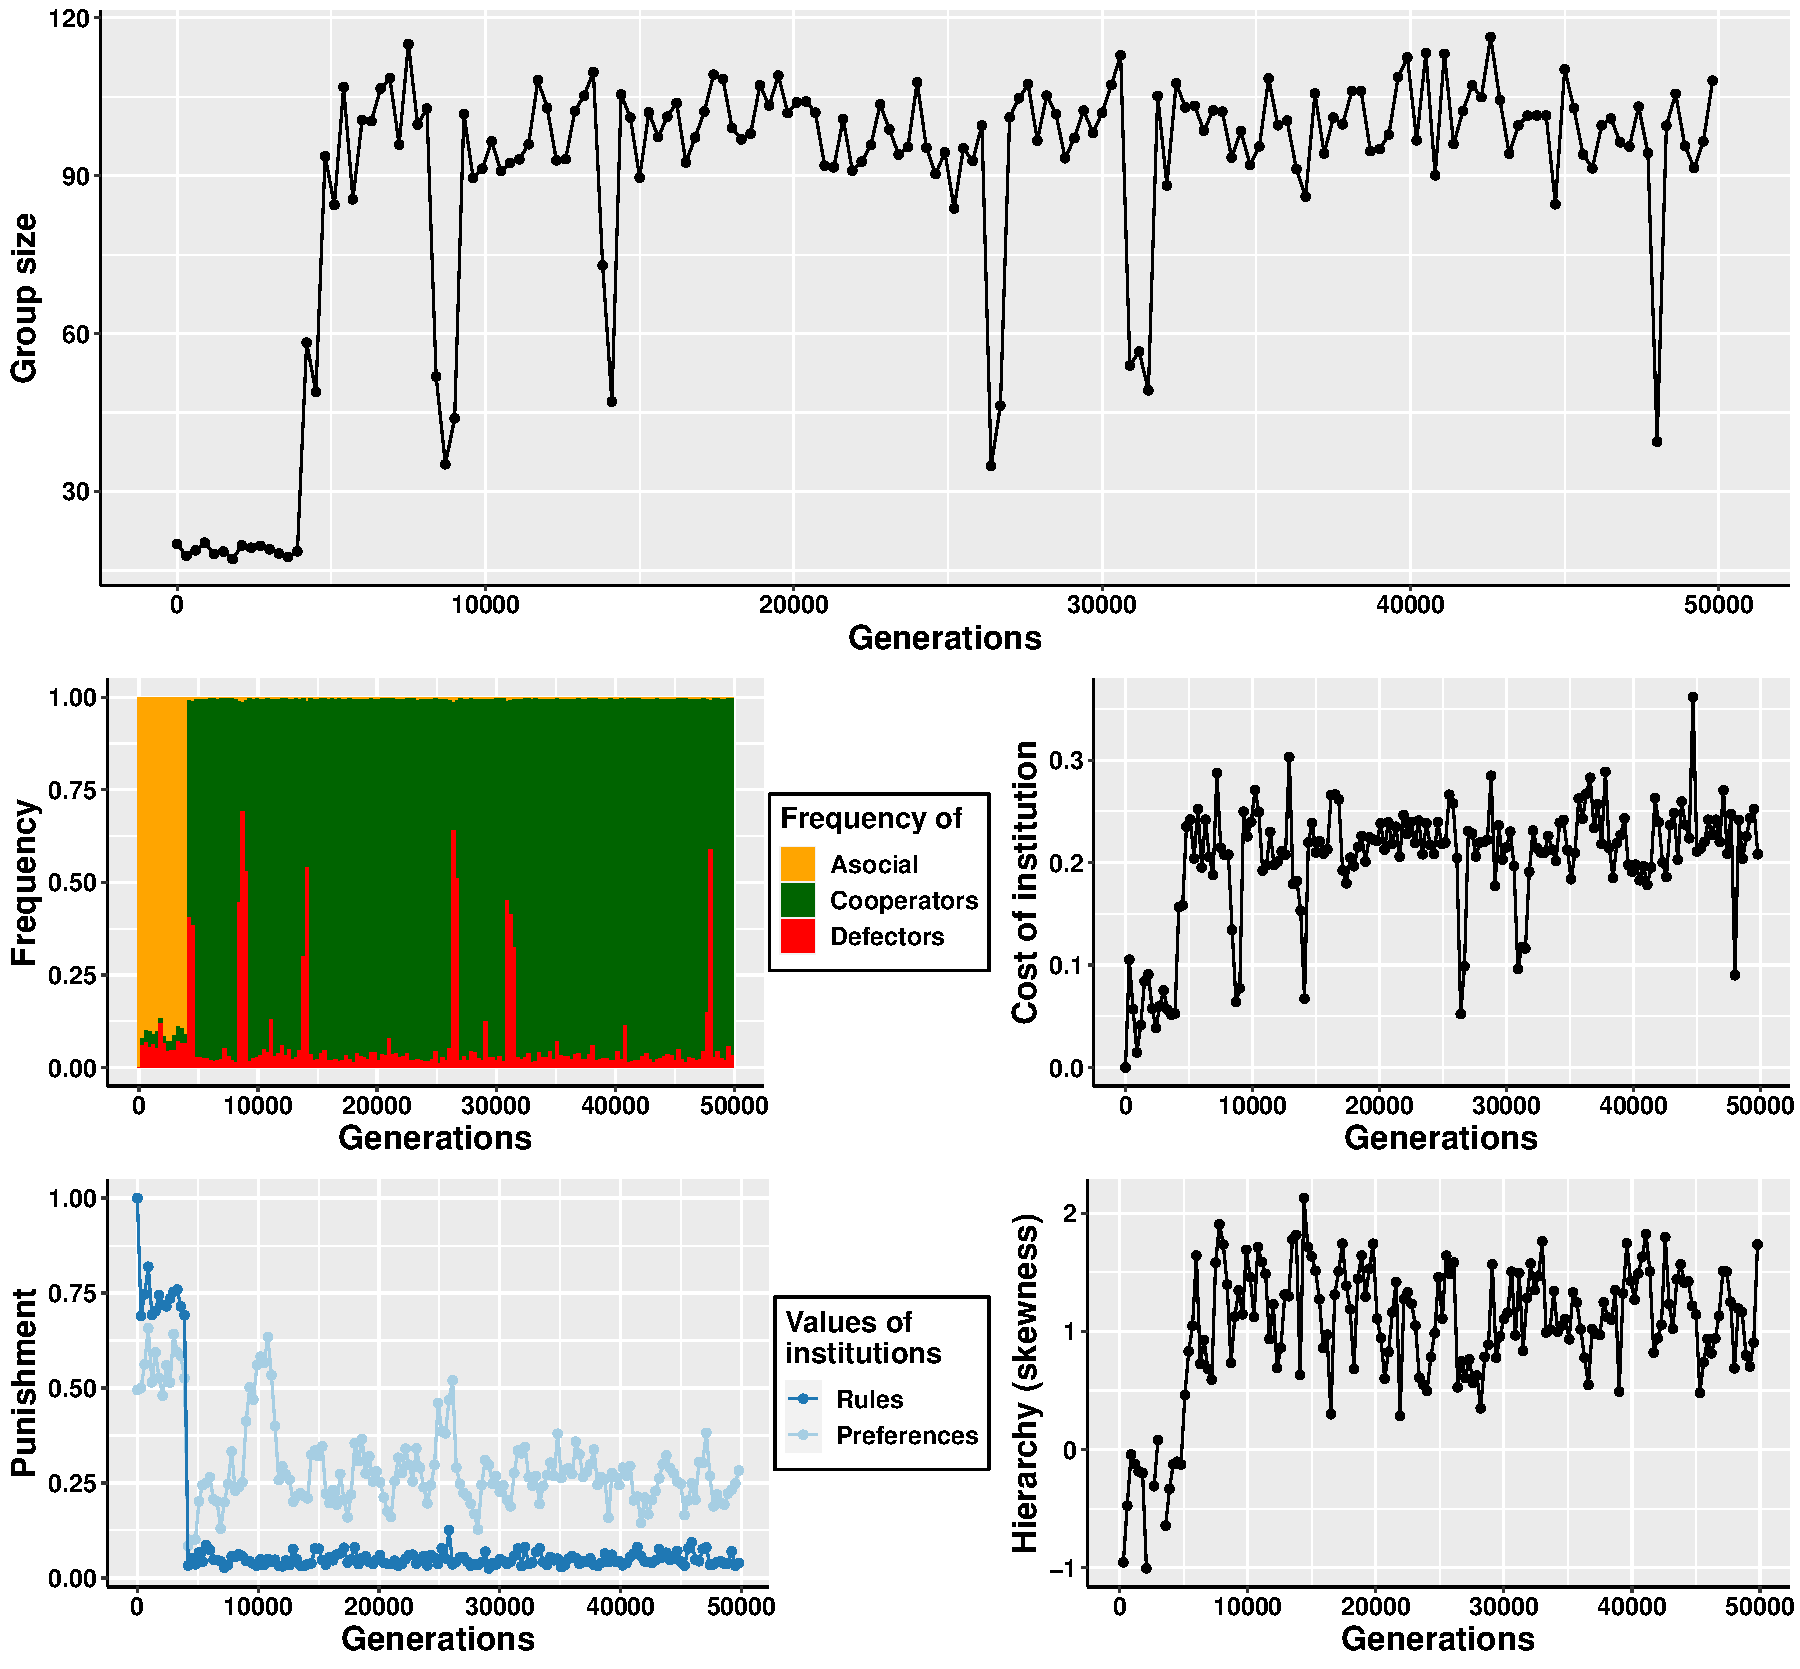
\includegraphics[width=0.8\linewidth]{Figures/pt_summary.pdf}
    \caption{Illustration of the evolution of cooperation, institutional rules, group size and hierarchy for the baseline model parameters.}
    \label{figBaseline}
\end{figure}

 The evolution of hierarchy occurs because the cost of playing the political game, $\iota_j(t_\mathrm{g})$, depends on the time taken for the group to reach consensus on the institutional rules, $t_{\mathrm{p}j}^*$ (Equation~\ref{eqnInstCost}). The time taken to reach consensus in this standard consensus formation model increases with group size \cite{Perret:2020:a}. Moreover, \cite{Perret:2020:a} demonstrates that in this model the rate of increase in consensus time with group depends upon the skew of $\alpha_{ij}$ values in the group. Groups with one or a small number of leaders -- individuals with $\alpha$ values much higher than the rest of their group -- increase their consensus time at a slower rate as their group size increases, compared to egalitarian groups which do not have this skew in the $\alpha$ traits of their individuals. As groups evolve cooperation-promoting institutions and grow in size from the benefits of cooperation, this creates selection pressure for hierarchy in order to reduce $\iota_j(t_\mathrm{g})$ (the mean value of this across groups is shown in the ``Cost of institution" graph in Figure~\ref{figBaseline}). Figure~\ref{figBaseline} shows that hierarchy evolves as groups start to create institutions and increase in size. As groups increase in size, social individuals in groups with hierarchy will have more offspring than social individuals in groups without hierarchy (Equations~\ref{eqnrc} and \ref{eqnrd}). This causes a spread of a positively-skewed distribution of $\alpha$ to different patches, with a minority of individuals evolving to act as leaders, and the rest as followers.

 As a control, we ran a version of the model where it was not possible for hierarchy to evolve. To do this, we initialised the population so that every individual had $\alpha=0.5$, and then did not allow mutations on this trait. In this case, social individuals were unable to form cooperation-promoting institutions as their group size increased. Specifically, in the control the mean frequency of cooperation over 50 000 generations and 10 replicates was 0.14, compared to 0.91 in the base model. Likewise, the average group size ($K_\mathrm{s}$) was 28 in the control, compared to 147 in the base model. This demonstrates that hierarchy is necessary to allow groups to maintain cooperation-promoting institutions as they grow in size, in order to reduce the cost of creating institutional rules via the political game of consensus formation. 

An important effect of hierarchy is that the institutional rules reached by consensus, $p_j(t_\mathrm{g})$, are biased in favour of the preferences of leaders. This follows from Equation~\ref{eqnUpdate}, where how much a listener changes their opinion depends on the difference in the $\alpha$ values of the speaker and listener. Moreover, leaders with high $\alpha$ values are more likely to be chosen as speakers in the first place (Equation~\ref{eqnProbSpeaker}). The ``Punishment'' graph in Figure~\ref{figBaseline} shows the average (mean across patches) difference between the mean value of the preference $p_{ij}$ of individuals on the patch, and the actual value of the institutional rules, $p_j(t_\mathrm{g})$, reached at consensus. This difference occurs because leaders $p$ preferences have the biggest effect on the consensus, and yet there are only a few such individuals on each patch. For the majority of individuals, who are followers, their $p_{ij}$ traits have much less effect on the consensus reached, and so they are under much less selection pressure. This allows them to drift to a certain degree. Supplementary Figure~S1 shows the correlation between the $\alpha_{ij}$ and $p_{ij}$ traits. The extent to which the consensus rules are dominated by the preferences of leaders is controlled by the parameter $x_\mathrm{thr}$, which we discuss in the next section. 

\subsection*{The effect of the threshold necessary to reach consensus, $x_\mathrm{thr}$}
The parameter $x_\mathrm{thr}$ specifies how close the opinions of social individuals have to be before consensus is reached, the political game ends, and $p_j(t_\mathrm{g})$ is set for their group (Equation~\ref{eqnConsensus}). It thus affects the time to reach consensus, and hence the cost of playing the political game. But moreover, it also affects the extent to which the consensus differs from the mean preference of the individuals. If $x_\mathrm{\theta}=1$ then consensus is reached immediately, and so $p_j(t_\mathrm{g})$ is then given by the mean $p_{ij}$ of all social individuals on the patch. Conversely, the lower the value of $x_\mathrm{thr}$ then the greater the number of discussion events that need to take place before $\sigma_x(t_{\mathrm{p}j}) < x_\mathrm{\theta}$ and consensus is reached. At each discussion event leaders are more likely to be chosen to speak than followers, and so the opinions of individuals are more likely to shift towards that of a leader than that of a follower. The more discussion events there are, the more times this shift in the opinion of followers is likely to occur. Empirically, we can think of $x_\mathrm{thr}$ as representing how difficult the political game is, i.e. how close the opinions of individuals have to be before they will accept the consensus rules. A lower value of $x_\mathrm{thr}$ represents a more difficult political game. This would correspond to the political game producing rules for an economic game that is very important for the material payoff of group members, and so each group member has a high stake. A larger value of $x_\mathrm{thr}$ represents an easier political game, i.e. rules that have relatively little effect on the material payoff of group members.



%\begin{figure}
    %\centering
    %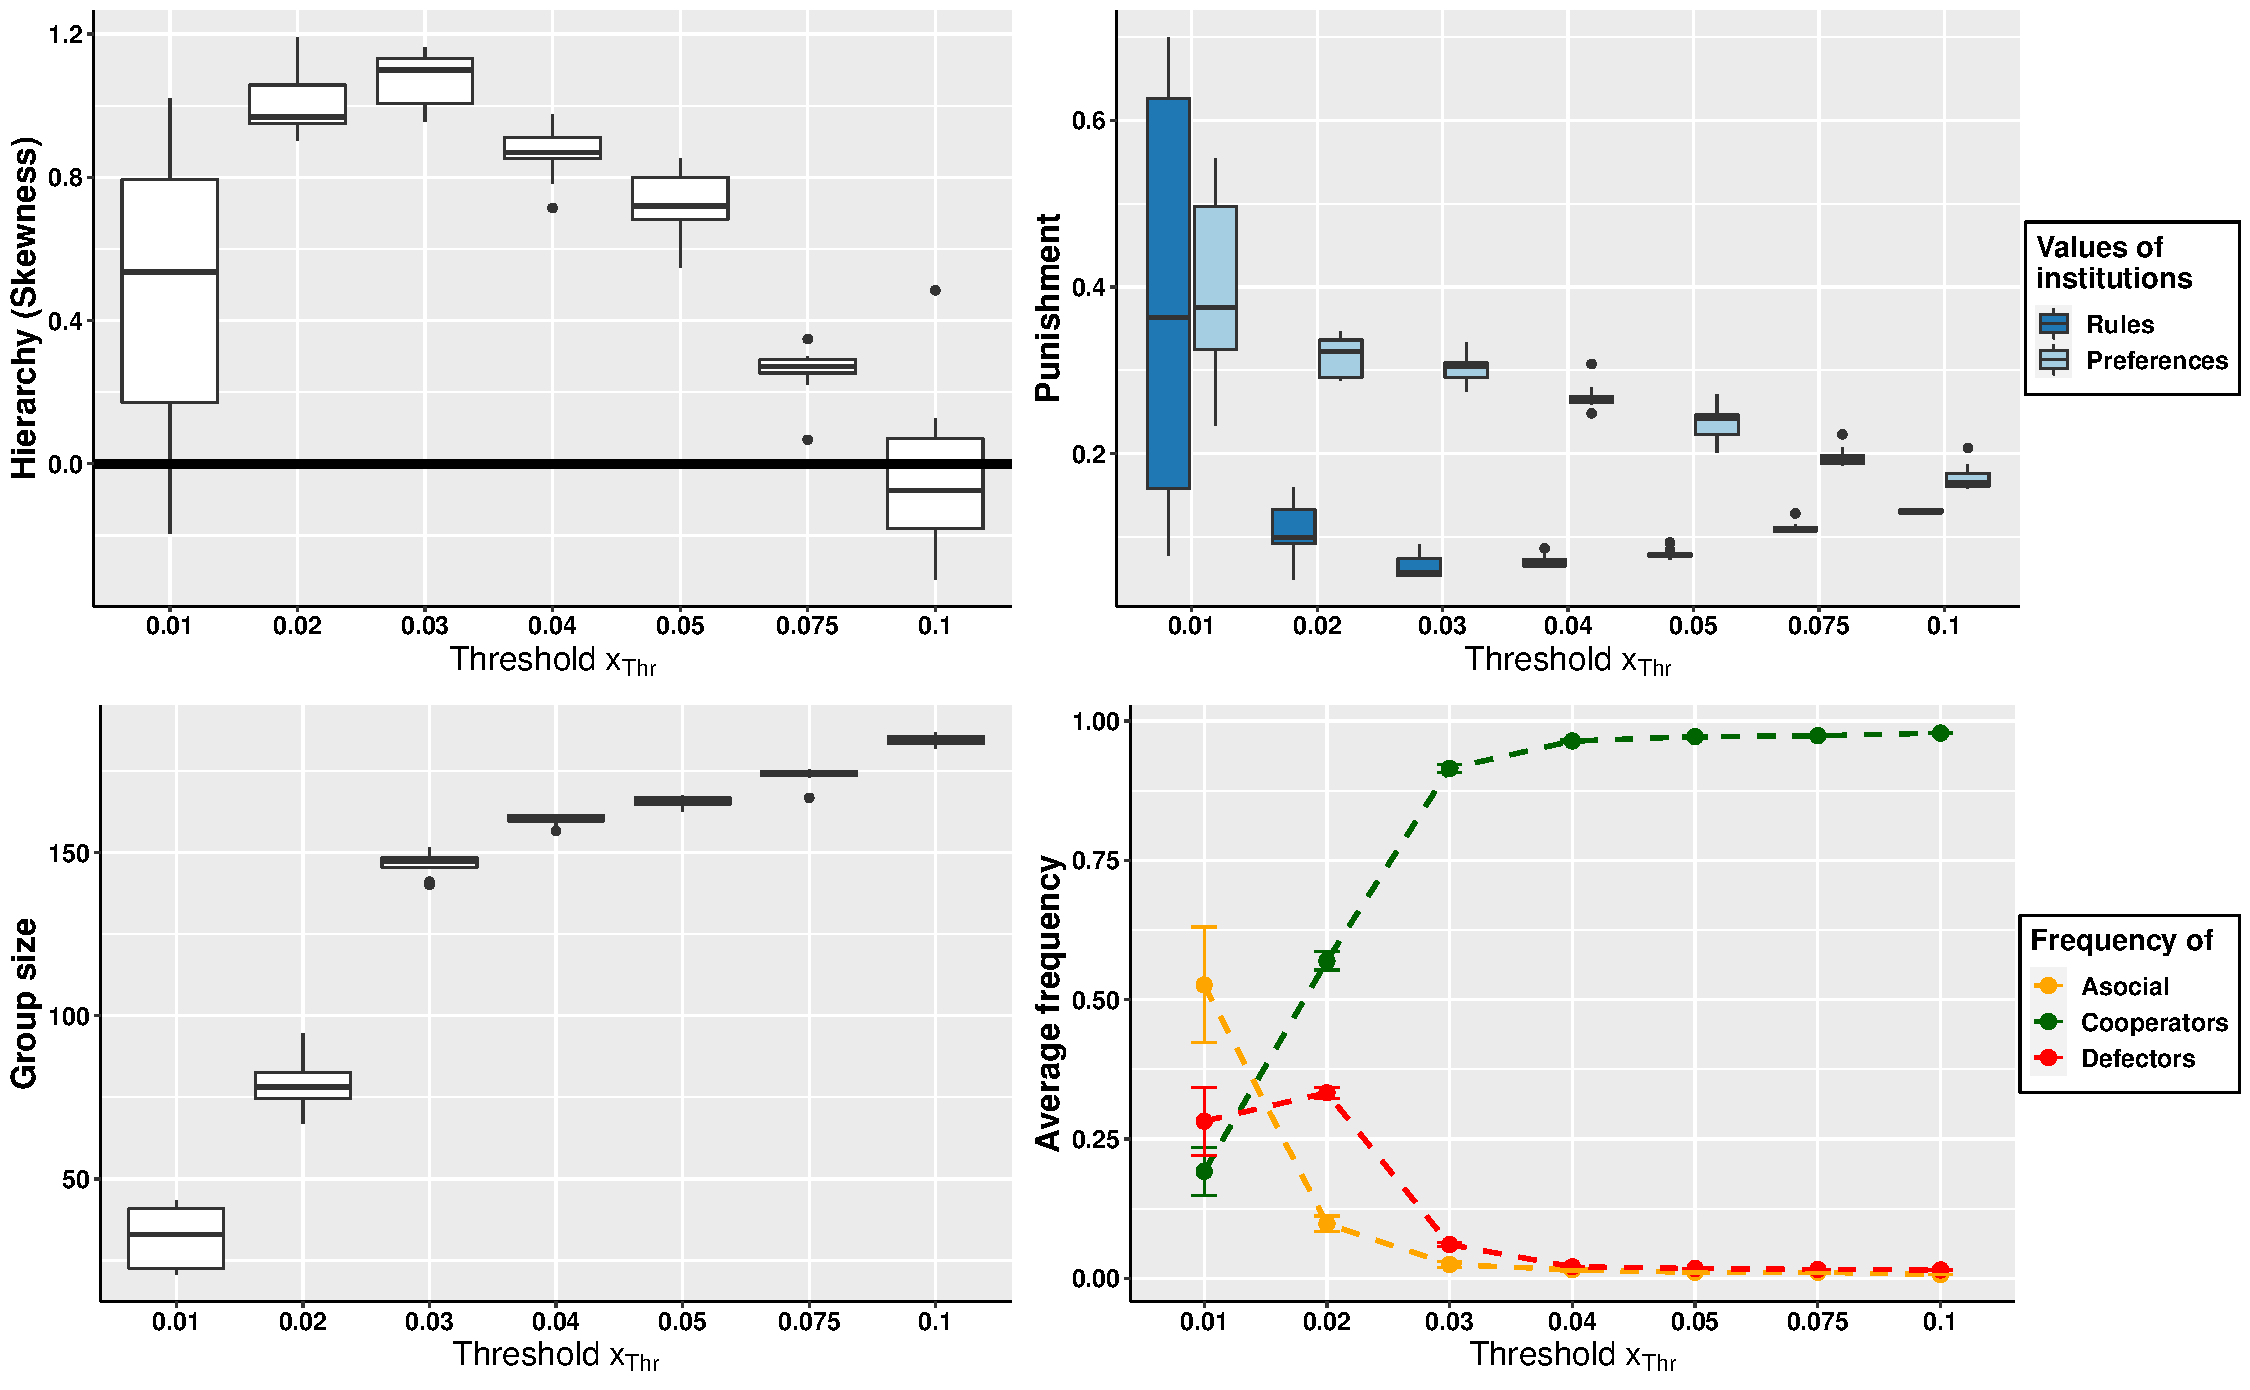
\includegraphics[width=0.8\linewidth]{Figures/pt_xThr.pdf}
    %\caption{}
    %\label{figXThr}
%\end{figure}

\begin{figure}, 
    \centering
    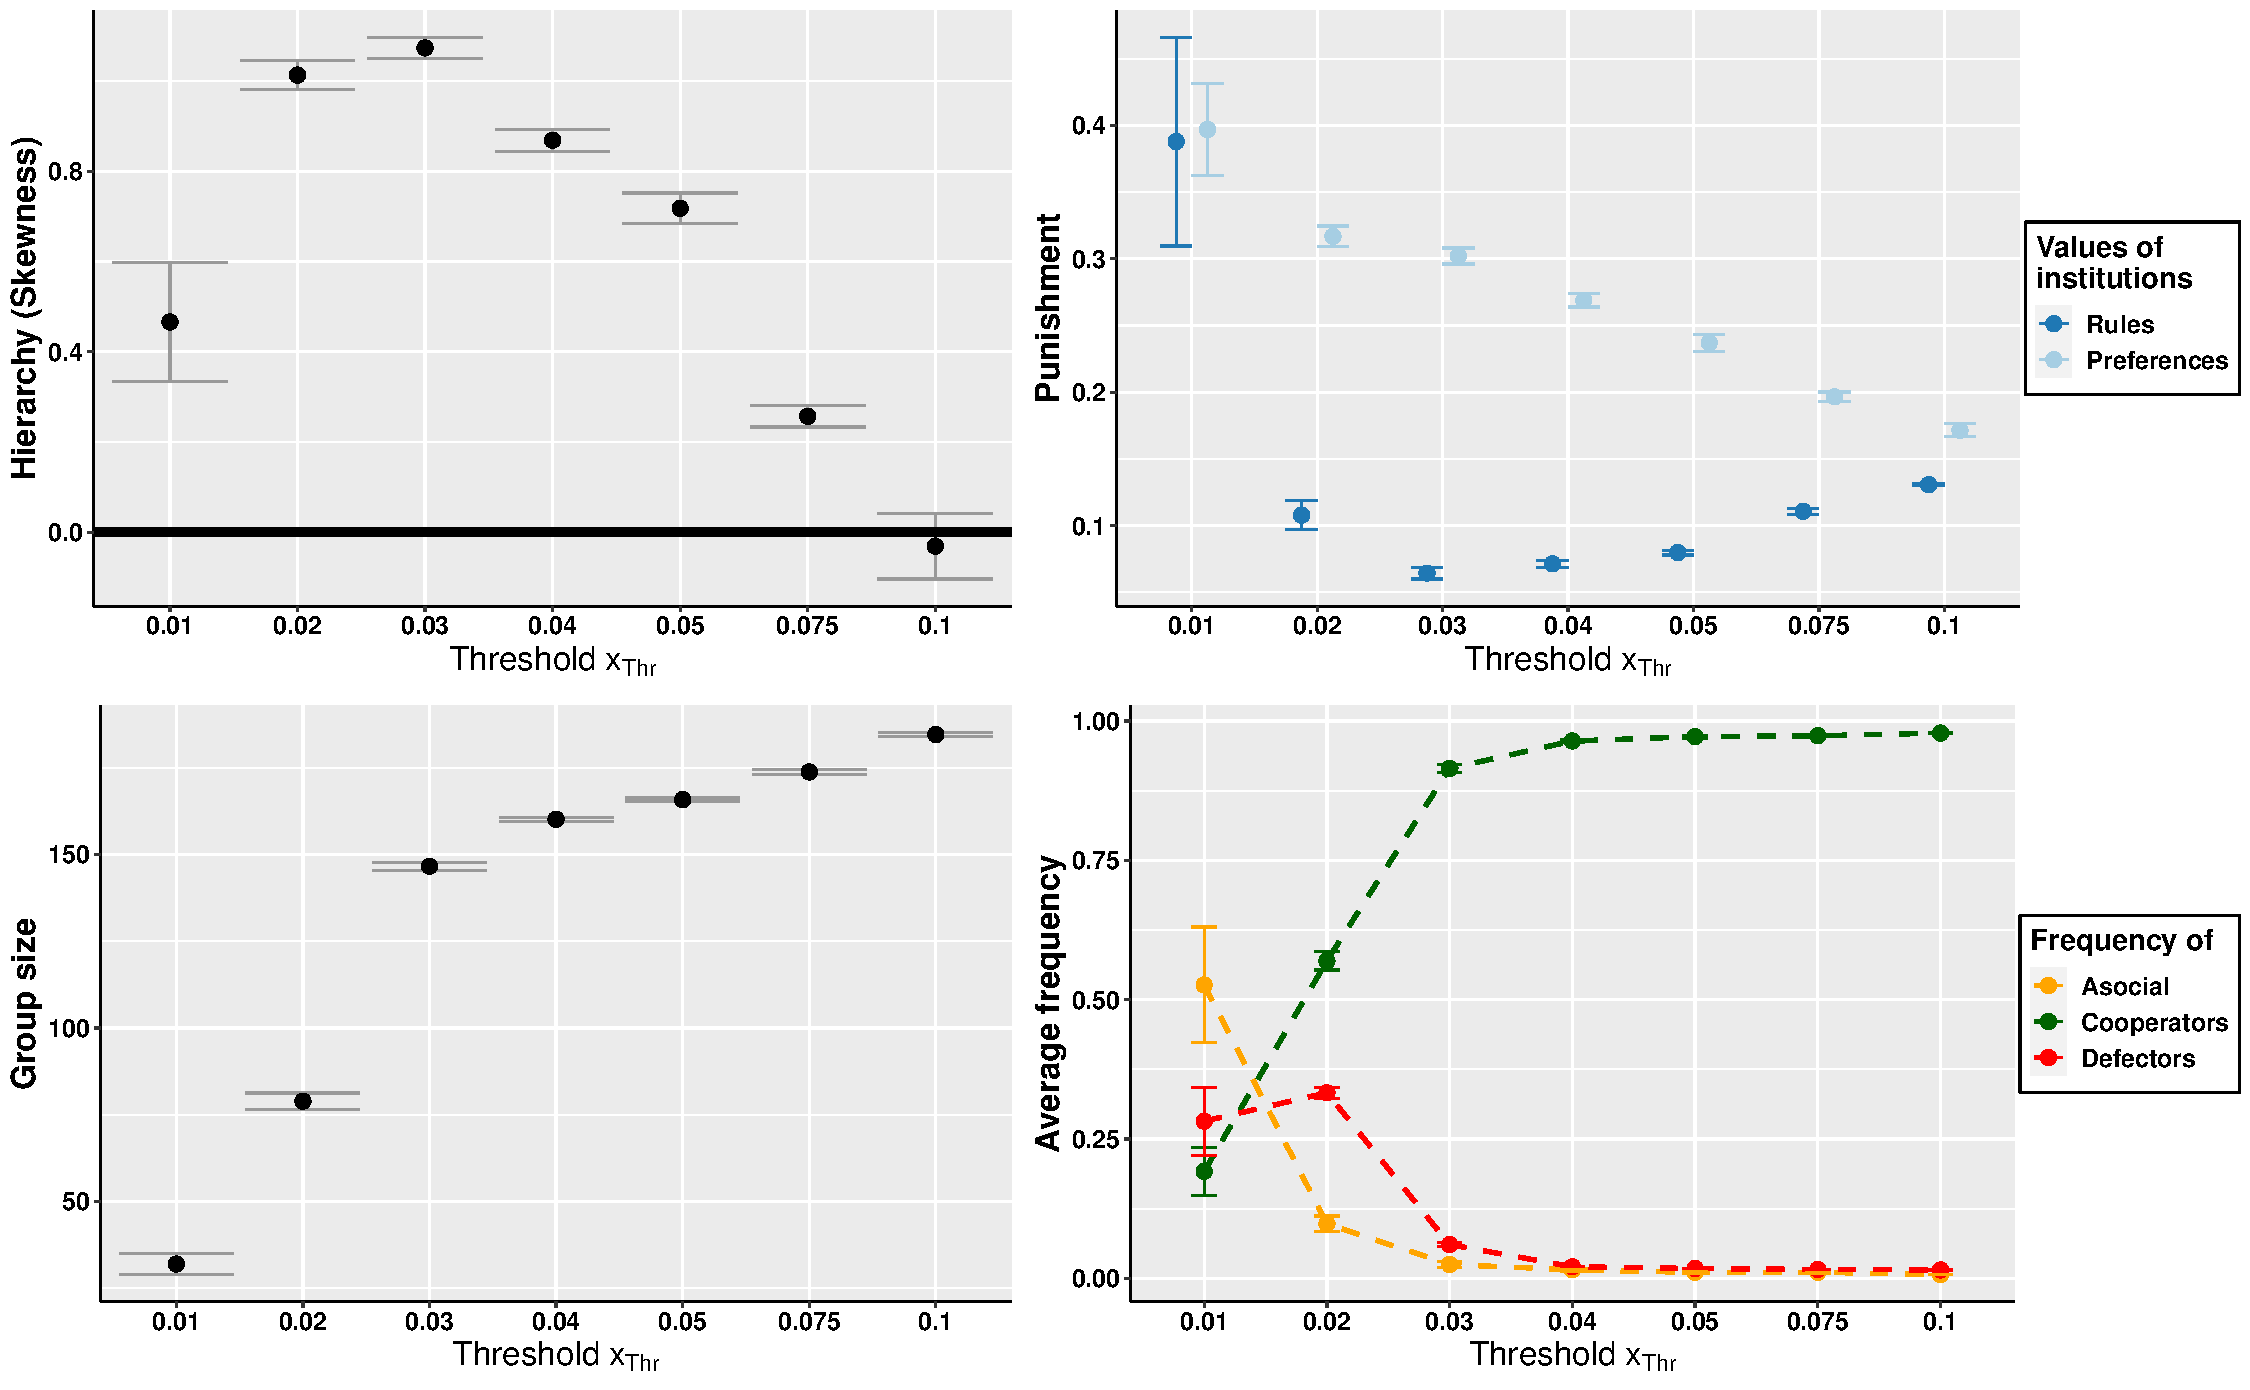
\includegraphics[width=0.8\linewidth]{Figures/pt_xThr_errorbar.pdf}
    \caption{The effect of varying how difficult the political game is, as determined by the threshold variance in individual opinions necessary to reach consensus, $x_\mathrm{thr}$. Each point represents the mean across 50 000 generations and 10 replicates. Error bars show the standard error.}
    \label{figXThr}
\end{figure}


Figure~\ref{figXThr} shows the effect of varying $x_\mathrm{thr}$ on the evolution of institutional rules, cooperation, group size and hierarchy. For intermediate values of $x_\mathrm{thr}$ we find the same results as in Figure~\ref{figBaseline} -- social individuals invade a population of asocials and establishing cooperation-promoting institutions, which lead to increasing group size and hierarchy. For high values of $x_\mathrm{thr}$, cooperation-promoting institutions evolve and drive an increase in group size, but we no longer see the evolution of hierarchy. In these cases, the time to reach consensus is fast even without hierarchy, leading to a low cost of playing the political game (Equation~\ref{eqnInstCost}) even in large egalitarian groups. There is thus not enough benefit to having hierarchy on the political game to lead to the evolution of a skewed distribution of $\alpha_{ij}$. On the other hand, for very low values of $x_\mathrm{thr}$ groups are unable to evolve cooperation-promoting institutions.

Figure~\ref{figGen_xThr} illustrates the dynamics of evolution during a run, and shows why this is the case. First, with a very low value of $x_\mathrm{thr}$, the time to reach consensus is high even in small groups. This makes it more difficult for social individuals to invade a population of asocials. More formally, the expected waiting time for socials to invade asocials in the stochastic increases as $x_\mathrm{thr}$ becomes smaller. This effect is illustrated in the ``Frequency'' graphs in Figure~\ref{figGen_xThr}. Second, once social individuals have invaded then for smaller values of $x_\mathrm{thr}$ they need more discussion events to reach consensus. As discussed above, the more discussion events there are, the more the rules reached at consensus are biased towards the preferences of small number of leaders. This means that the preferences of followers matter less and so are subject to drift, as illustrated in the ``Punishment'' graph in Figure~\ref{figGen_xThr}. However, this drift in the preferences of the majority of group members then weakens competition between groups, which occurs via differential migration. In the baseline model, \cite{Powers:2013:a}, individuals in groups that invest just enough into punishment to incentivise cooperation produce more offspring, and then export their preferences for these ``optimal'' institutional rules to other groups. This mechanism functions effectively when migrants have an effect on the institutional rules in their new groups. This was the case in \cite{Powers:2013:a}, where the institutional rules were formed by taking the mean preference of the group members. This is also the case for medium and high $x_\mathrm{thr}$ in our model. However, for low $x_\mathrm{thr}$, followers -- who make up the majority of migrants -- have little effect on the consensus, and their preferences drift. This dilutes competition between the institutions of different groups, and leads to groups investing too little into punishment to incentivise cooperation. When the majority of individuals have little to no say in the institutional rules then the group loses the benefits of the ``wisdom of the crowd'' \cite{Ober:2008:a}, and so can fail to move to more optimal rules. 

\begin{figure}
    \centering
    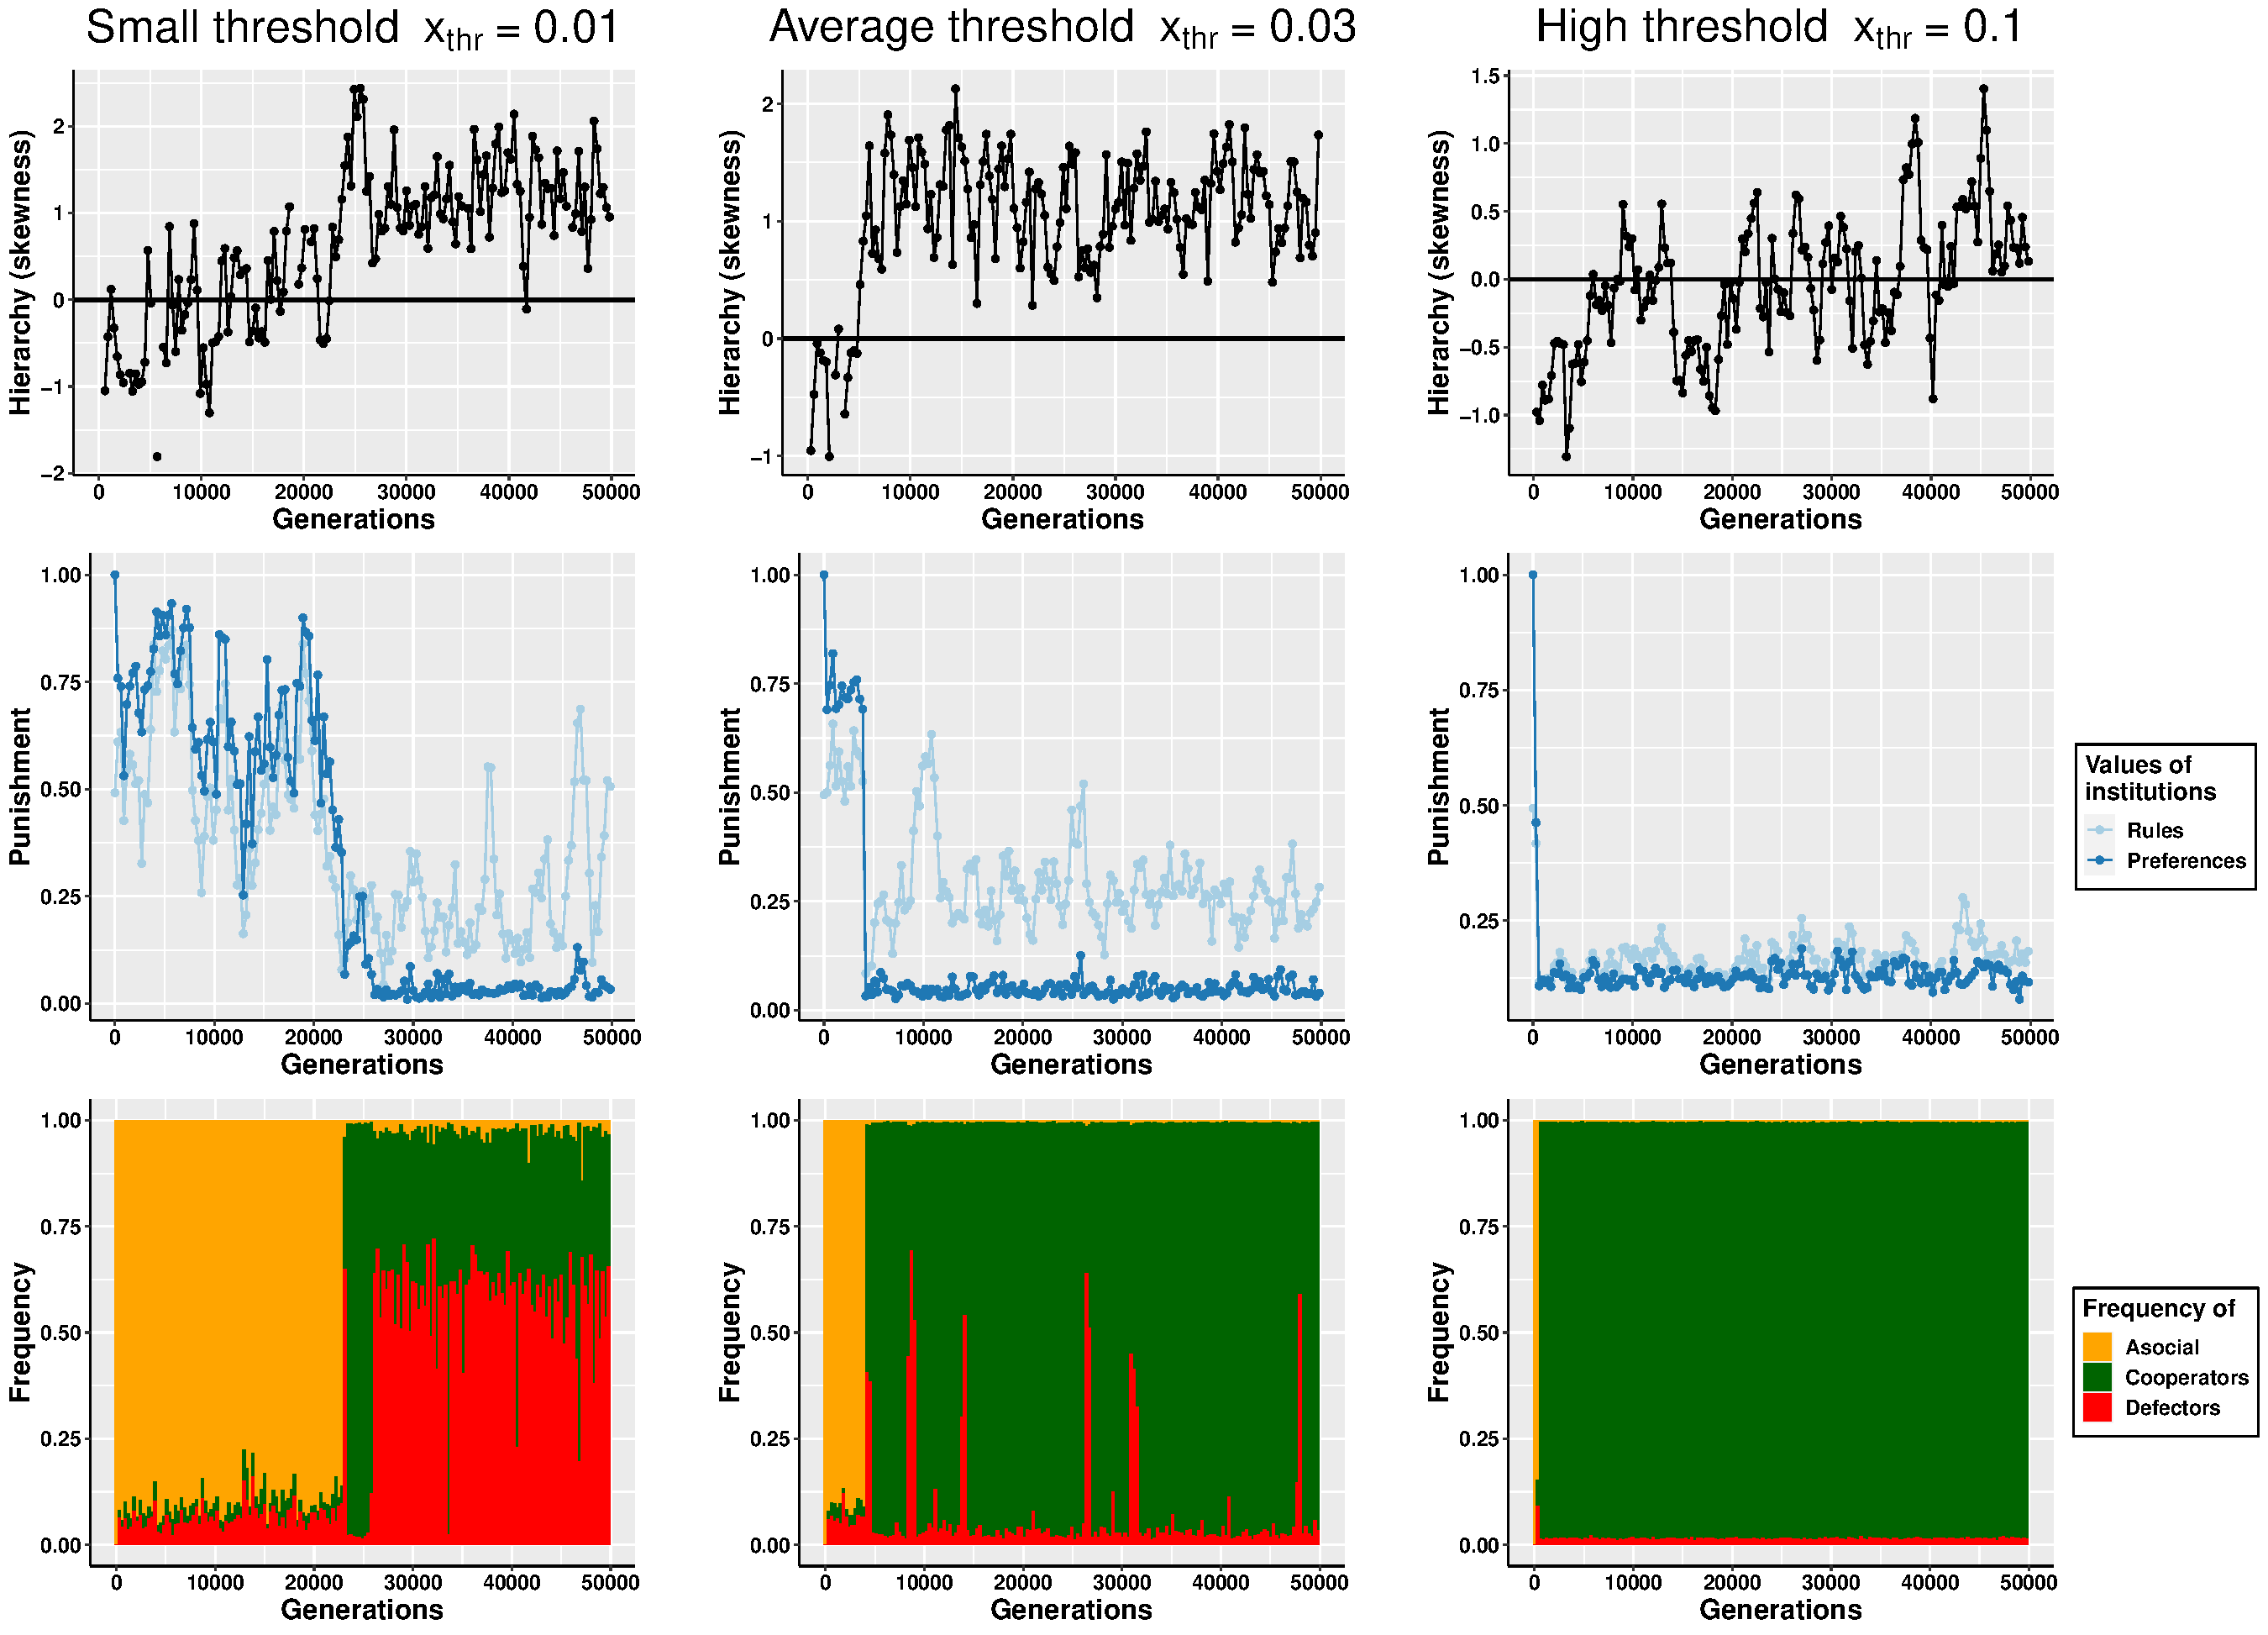
\includegraphics[width=0.8\linewidth]{Figures/pt_gen_xThr.pdf}
    \caption{Illustration of the evolutionary dynamics for hard, medium and easy political games (low, average and high $x_\mathrm{thr}$).}
    \label{figGen_xThr}
\end{figure}

\subsection*{Sensitivity to parameters}
Supplementary Figure~S2 shows the effect of varying the benefit of cooperation, $B$. For low $B$, institutional rules are selected that invest a greater proportion of the public good into punishment. However, this greater investment leads to a smaller increase in $K_{\mathrm{s}}$ and hence a smaller group size. On the other hand, for a larger $B$ a smaller proportion of the public good is invested into punishment -- but this smaller proportion is still larger in absolute terms and so can maintain cooperation while allowing groups to grow even larger. The institutional rules thus evolve to match the efficiency of cooperation.

The effects of varying the initial group size, $K_\mathrm{a}$, were studied in \cite{Powers:2013:a}. This must be small to allow social individuals to invade a population of asocials. However, once socials have invaded, their institutionally-supported punishment can maintain cooperation as groups become much larger. The consensus time cost scalar, $I$, is multiplied by the consensus time to translate the time into a fitness cost. If this is 0 then cooperation-promoting institutions evolve without hierarchy. Conversely, if it is very large then cooperation-promoting institutions cannot evolve, because the fitness cost of having an institution is too large. The number of listeners during a discussion event, $N_\mathrm{l}$, affects how quickly a group reaches consensus. For larger $N_\mathrm{l}$, consensus is reached quicker \cite{Perret:2022:a}. Empirically, we would expect $N_\mathrm{l}$ to be larger if groups have more effective communication technology (e.g. writing), or if the political game is itself structured to facilitate opinion formation, e.g. through individuals meeting in organised assemblies to exchange views.  

\section*{Discussion}
We have demonstrated that under a wide range of conditions the evolution of cooperation-promoting institutions leads to the evolution of hierarchy. This is because cooperative groups grow in size from the benefits of their cooperative activities. However, as they grow in size then the process of negotiating and forming their institutional rules -- their political game -- becomes more costly. This scalar stress \cite{Johnson:1982:a} favours the evolution of hierarchy to reduce the cost of rule formation. The ``Iron Law of Oligarchy'' \cite{Michels:1911:a} states that it is inevitable that initially small and democratic organisations will transition to oligarchy (extreme hierarchy) as they grow in size, due to the increasing costs of organisation in large groups. Our model formalises this, and suggests that institutional rule formation is a key and general example of an organisational problem that leads to hierarchy, giving rise to the ``Iron Law of Institutions''.

An important empirical case that fits the predictions of our model is the growth in group size during the Neolithic Demographic Transition \cite{Bocquet-Appel:2011:a}. During this period population size drastically increased due to the origin of agriculture. At the same time, new social problems would have arisen that required institutional rules, such as development and management of irrigation systems shared by many individuals \cite{Hunt:1988:a,Trawick:2001:a,Janssen:2012:a,Carballo:2014:a}. Moreover, during this time there is strong evidence that groups transitioned from egalitarian to hierarchical organisation  \cite{Boehm:1999:a,Price:1995:a,Price:2010:a}. Our model suggests that the need to form intuitions to regulate more complex activities among greater numbers of individuals would would lead to the evolution of hierarchy, in order to reduce the costs of institution formation. It thus explains why cooperation-promoting institutions, increasing group size, and hierarchy go hand-in-hand with the origin of agriculture. 

We have modelled the evolution of informal leadership, in which individuals evolve to become more like leaders or more like followers. This evolution of leadership based on individual traits can help to explain the origin of hierarchy. However, as our results show, this informal leadership has limitations as the political game becomes more difficult ($x_\mathrm{thr}$ becomes smaller). Formal leadership, where there is a single designated leader in a group, may overcome this. For example, a designated leader may learn rules from the leaders of other successful groups, avoiding the need for successful rules to spread via differential migration, with the problems that entails for difficult political games. Indeed, as societies grew larger they formalised leadership into a hereditary position (chiefdoms), and ultimately multiple layers of hierarchy (states).
%\begin{figure} 
    %\centering
    %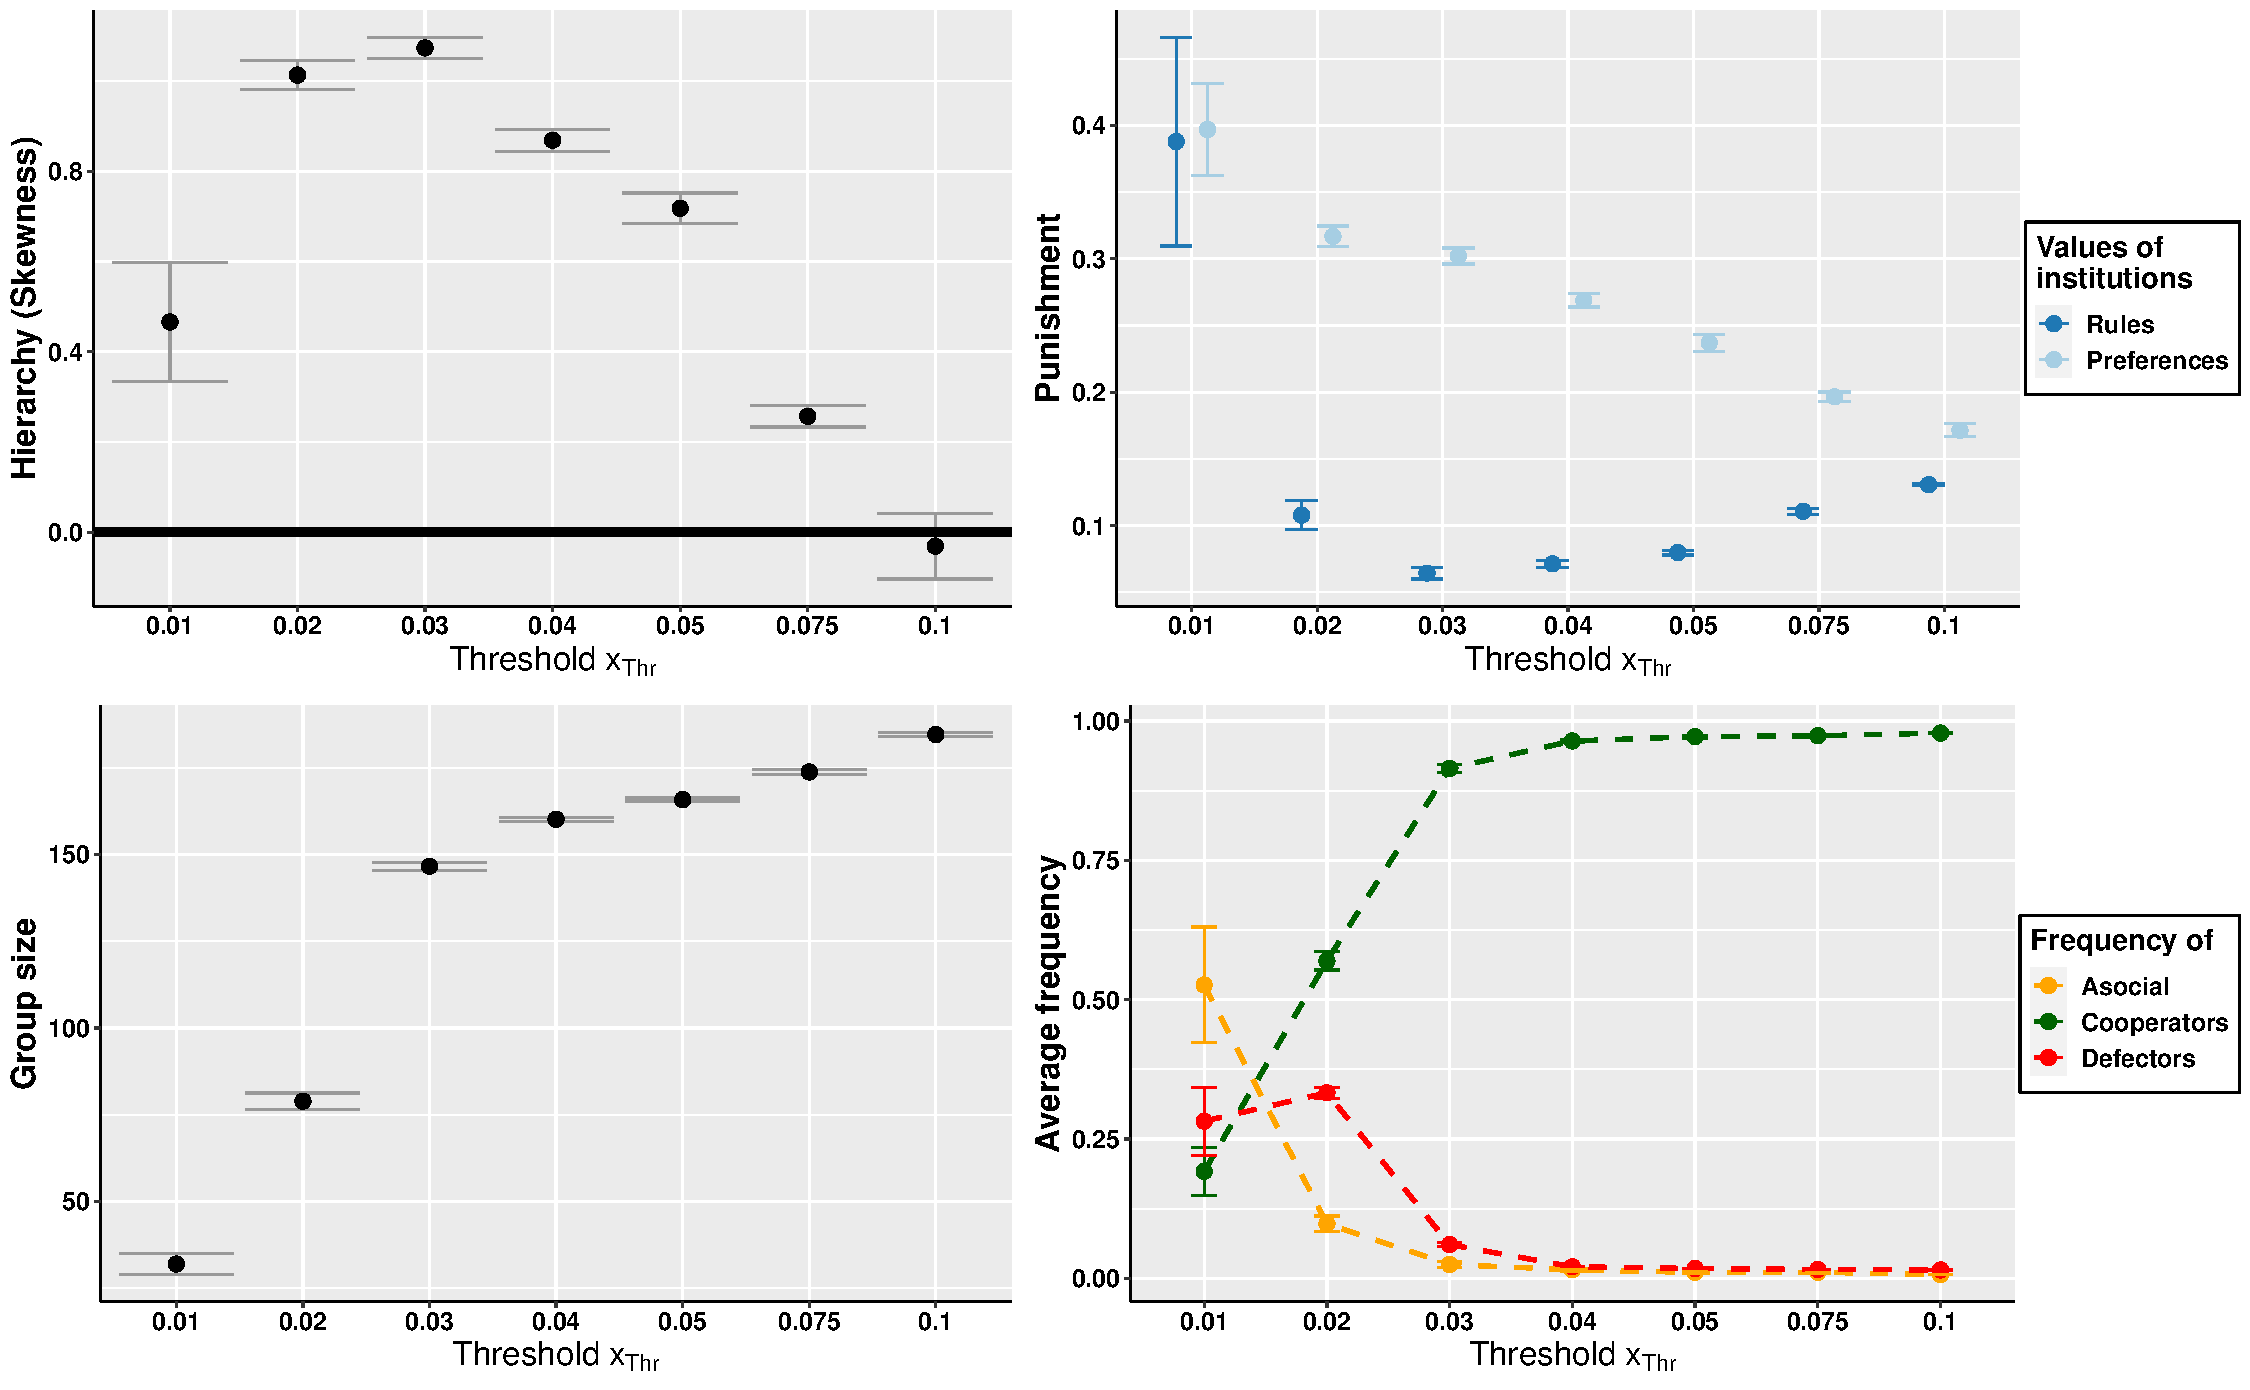
\includegraphics[width=0.8\linewidth]{Figures/pt_xThr_errorbar.pdf}
    %\caption{}
    %\label{fig:xThr}
%\end{figure}






%\subsection*{The effect of cost of institution}

%\begin{figure}
    %\centering
    %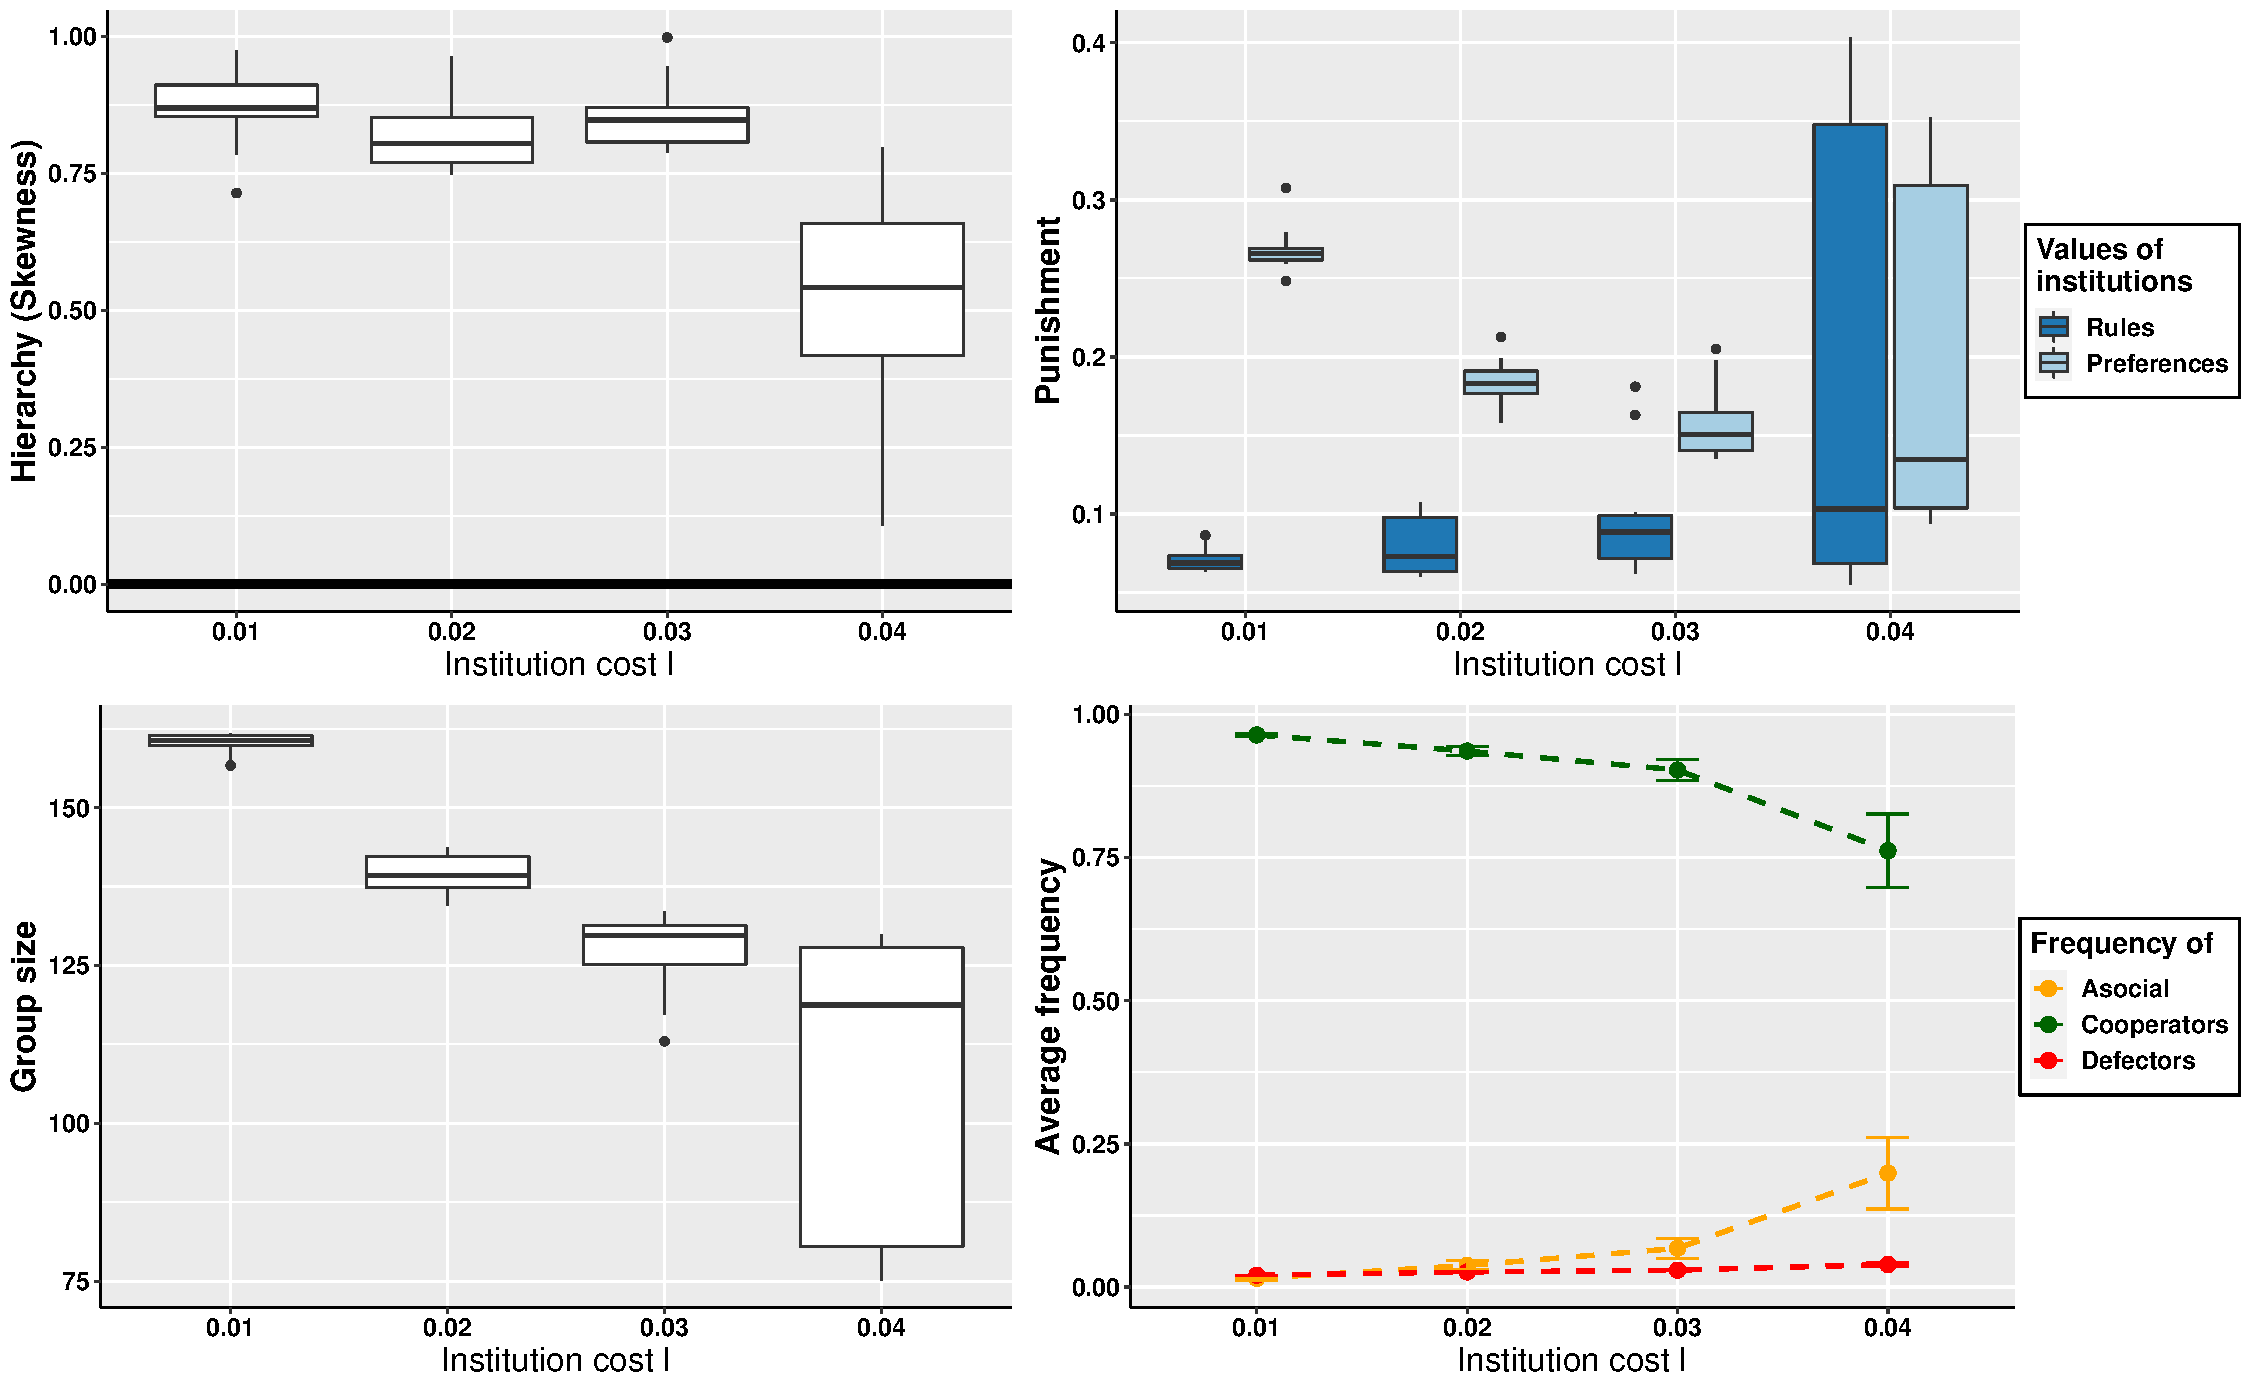
\includegraphics[width=0.8\linewidth]{Figures/pt_instCost.pdf}
    %\caption{}
    %\label{figI}
%\end{figure}

%\subsection*{Benefit cost ratio}

%\begin{figure}
    %\centering
    %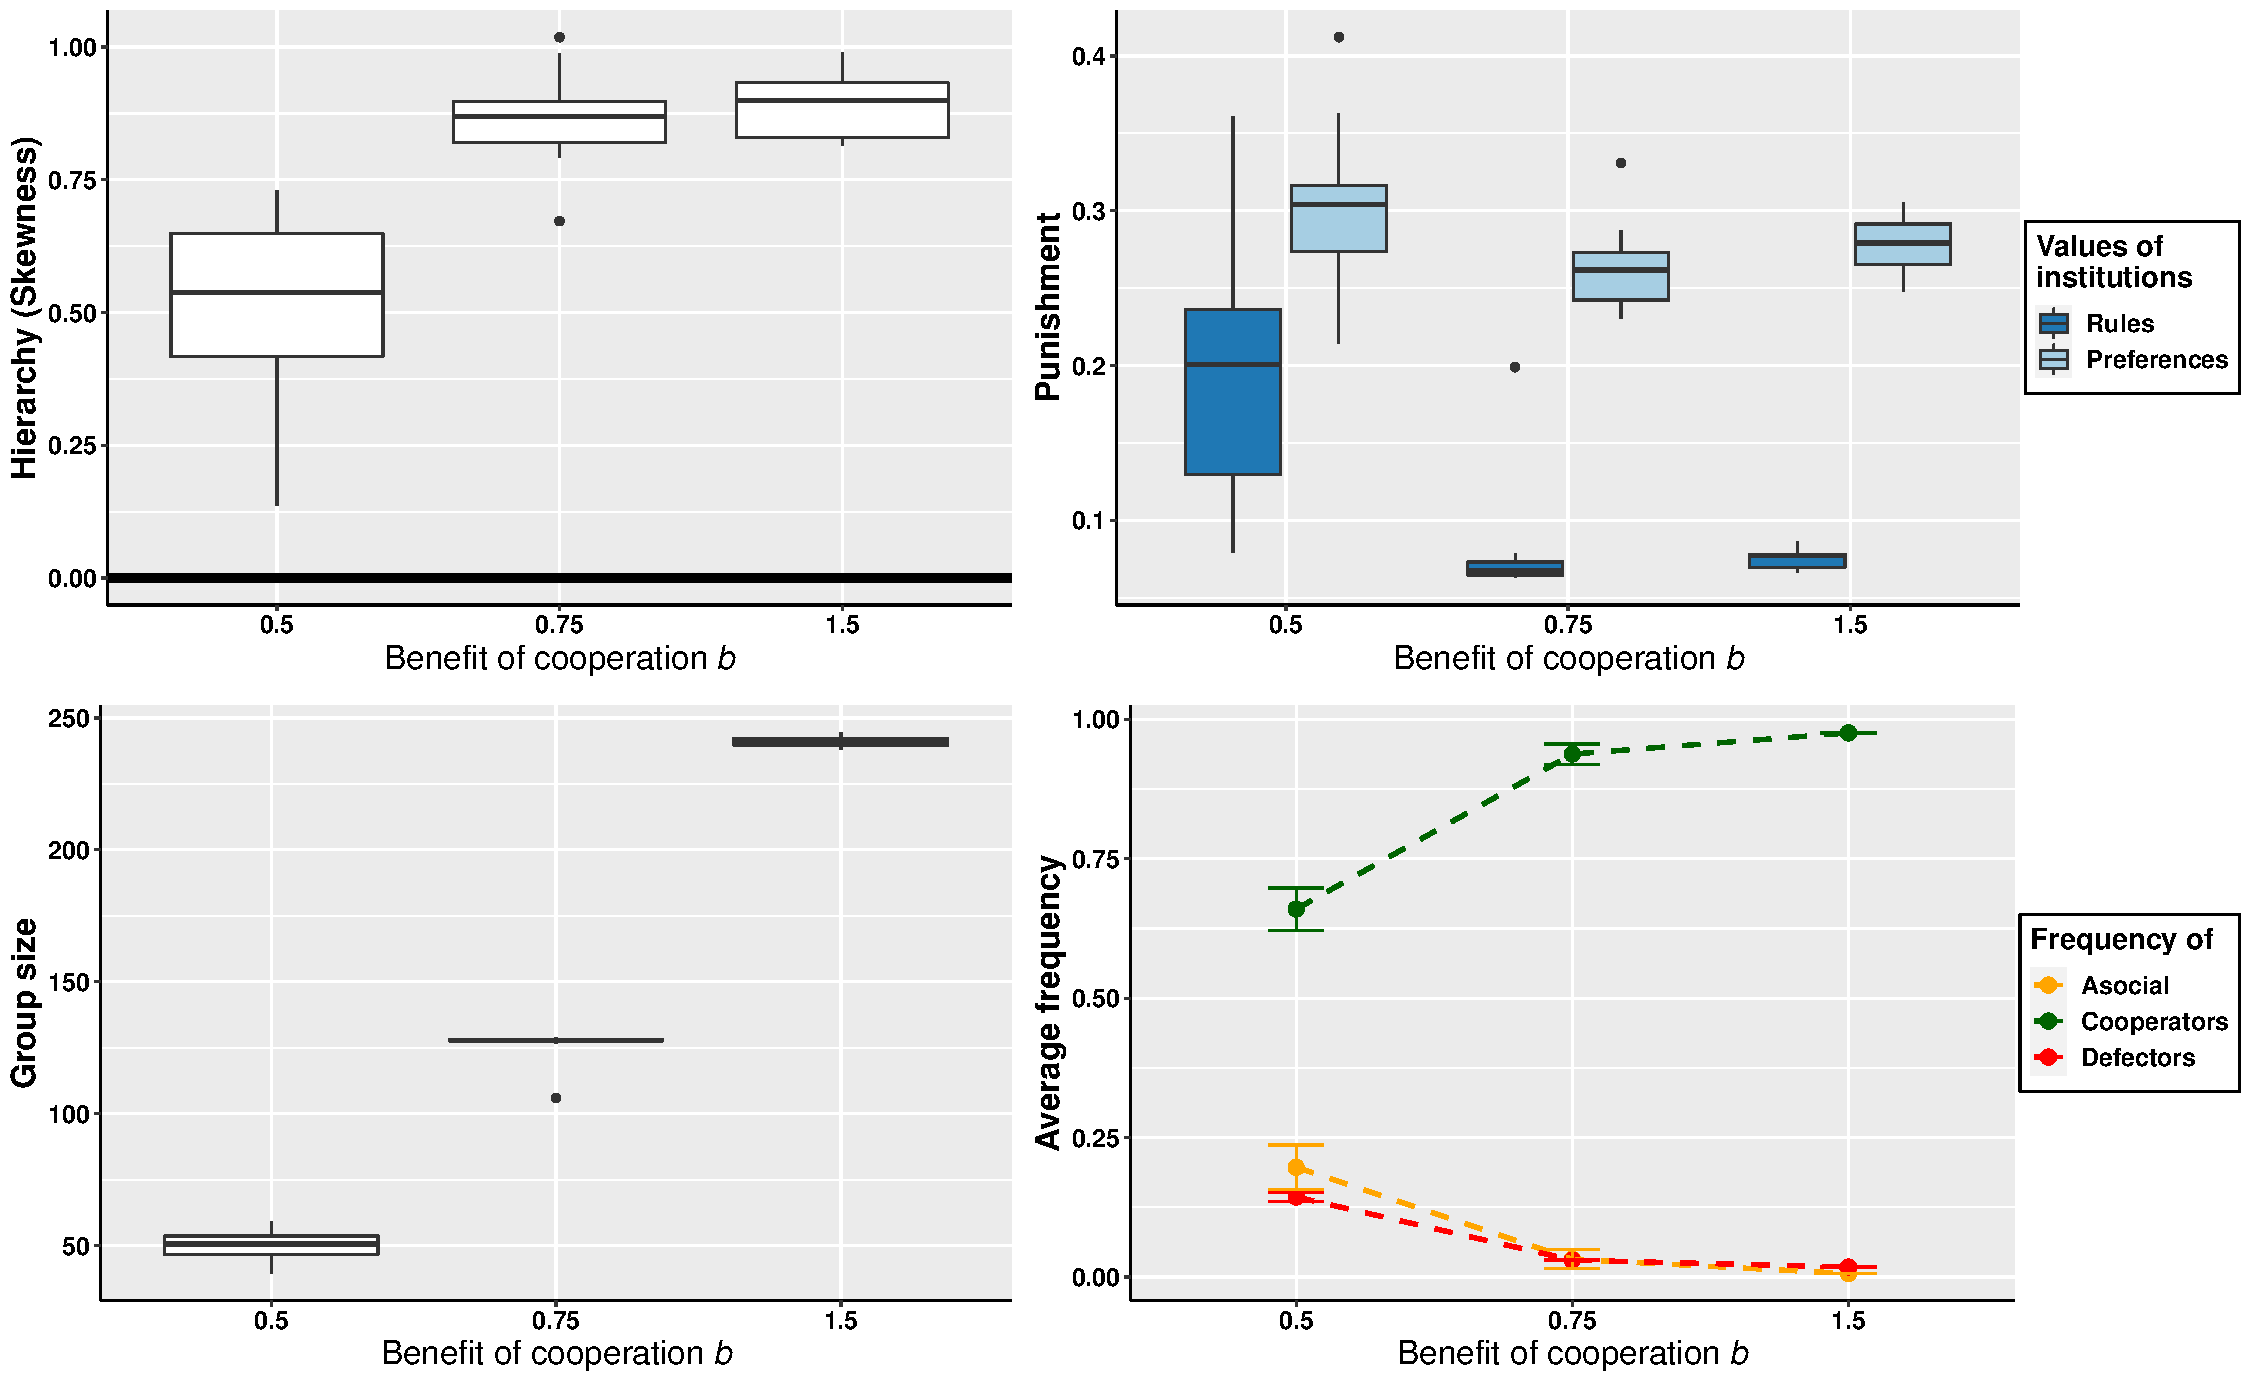
\includegraphics[width=0.8\linewidth]{Figures/pt_coopB.pdf}
    %\caption{}
    %\label{figB}
%\end{figure}









\textbf{Author contributions}: STP, CP and TC designed the study, STP implemented the model, STP and CP conducted the analysis, STP, CP and TC wrote the manuscript.

\textbf{Author Information:} The authors declare no competing financial interests. Correspondence and requests for materials should be addressed to STP (e-mail: S.Powers@napier.ac.uk).

\textbf{Data availability statement}: The code is available online at\\ ``https://github.com/CedricPerret'' in the project ``TerCirNet''.

\textbf{Funding statement:} C.P. \& T.E.C. are supported by funding awarded to T.E.C. from the European Research Council (ERC) under the European Union’s Horizon 2020 research and innovation programme (\textit{The Cultural Evolution \& Ecology of Institutions}, Grant Agreement 716212).



\bibliographystyle{RS.bst}
\bibliography{references.bib}


\end{linenumbers}

\end{document}
